% CVPR 2024 Paper Template; see https://github.com/cvpr-org/author-kit

\documentclass[10pt,twocolumn,letterpaper]{article}

%%%%%%%%% PAPER TYPE  - PLEASE UPDATE FOR FINAL VERSION
\usepackage{cvpr}              % To produce the CAMERA-READY version
%\usepackage[review]{cvpr}      % To produce the REVIEW version
%\usepackage[pagenumbers]{cvpr} % To force page numbers, e.g. for an arXiv version
\usepackage{diagbox}
\usepackage{graphicx}
\usepackage{amsmath}
\usepackage{amssymb}
\usepackage{booktabs}
\usepackage[dvipsnames]{xcolor}
\usepackage{flexisym}
\usepackage{amsmath}
\usepackage{multirow}
\usepackage{tabularx}
\usepackage{enumitem}

\usepackage{amssymb}% http://ctan.org/pkg/amssymb
\usepackage{pifont}% http://ctan.org/pkg/pifont
\newcommand{\cmark}{\ding{51}}%
\newcommand{\xmark}{\ding{55}}%

% Import additional packages in the preamble file, before hyperref
%
% --- inline annotations
%
\usepackage[dvipsnames]{xcolor}
\newcommand{\red}[1]{{\color{red}#1}}
\newcommand{\todo}[1]{{\color{red}#1}}
\newcommand{\TODO}[1]{\textbf{\color{red}[TODO: #1]}}
% --- disable by uncommenting  
% \renewcommand{\TODO}[1]{}
% \renewcommand{\todo}[1]{#1}



% It is strongly recommended to use hyperref, especially for the review version.
% hyperref with option pagebackref eases the reviewers' job.
% Please disable hyperref *only* if you encounter grave issues, 
% e.g. with the file validation for the camera-ready version.
%
% If you comment hyperref and then uncomment it, you should delete *.aux before re-running LaTeX.
% (Or just hit 'q' on the first LaTeX run, let it finish, and you should be clear).
\definecolor{cvprblue}{rgb}{0.21,0.49,0.74}
\usepackage[pagebackref,breaklinks,colorlinks,citecolor=cvprblue]{hyperref}

%%%%%%%%% PAPER ID  - PLEASE UPDATE
\def\paperID{3} % *** Enter the Paper ID here
\def\confName{CVPR}
\def\confYear{2024}

%%%%%%%%% TITLE - PLEASE UPDATE
\title{MonoSelfRecon: Purely Self-Supervised Explicit Generalizable 3D Reconstruction of Indoor Scenes from Monocular RGB Views}

%%%%%%%%% AUTHORS - PLEASE UPDATE
\author{Runfa Li\textsuperscript{1} \quad
%{\tt\small rul002@ucsd.edu}
Upal Mahbub\textsuperscript{2} \quad
Vasudev Bhaskaran\textsuperscript{2} \quad
Truong Nguyen\textsuperscript{1} \quad
\\
\textsuperscript{1}UC San Diego \quad
\textsuperscript{2}Qualcomm %Technologies Inc.
}



\begin{document}
\maketitle
\begin{abstract}
 Current monocular 3D scene reconstruction (3DR) works are either fully-supervised, or not generalizable, or implicit in 3D representation. We propose a novel framework - \textbf{MonoSelfRecon} that for the first time achieves \textbf{explicit 3D mesh} reconstruction for \textbf{generalizable} indoor scenes with monocular RGB views by purely \textbf{self-supervision} on voxel-SDF (signed distance function). MonoSelfRecon follows an Autoencoder-based architecture, decodes voxel-SDF and a generalizable Neural Radiance Field (NeRF), which is used to guide voxel-SDF in self-supervision. We propose novel self-supervised losses, which not only support pure self-supervision, but can be used together with supervised signals to further boost supervised training. Our experiments show that "MonoSelfRecon" trained in pure self-supervision outperforms current best self-supervised indoor depth estimation models and is comparable to 3DR models trained in fully supervision with depth annotations. MonoSelfRecon is not restricted by specific model design, which can be used to any models with voxel-SDF for purely self-supervised manner. %\footnote{Datasets  were  downloaded  and  evaluated  solely  by  the researchers from UC San Diego.}
\end{abstract}    
\section{Introduction} \label{intro}


With the recent development of deep generative models, speech synthesis has seen an extraordinary progress. Among the conventional speech synthesis methods, WaveNets~\cite{oord2016wavenet} were demonstrated to generate high-fidelity audio samples in an autoregressive manner yet suffering from prohibitively expensive computational costs. In contrast, non-autoregressive approaches such as flow-based and GAN-based models~\cite{prenger2019waveglow,jang2021univnet,kong2020hifi,huang2021multi} were also proposed to generate speech audios with satisfactory speed. However, these models were still criticized for other problems, e.g., the limited sample quality or sample diversity \cite{xiao2021tackling}.

In speech synthesis, our goal is mainly two-fold:
\begin{itemize}
    \item High-quality: generating high-quality speech is a challenging problem especially when the sampling rate of an audio is high. It is vital to reconstruct details at different timescales for waveforms of highly variable patterns.
    \item Fast: high generation speed is essential when considering real-time speech synthesis. This poses a challenge for all high-quality neural synthesizers.
\end{itemize}

As a blossoming class of generative models, denoising diffusion probabilistic models (DDPMs)~\cite{ho2020denoising,song2020denoising,lam2022bddm,liu2022pseudo} has emerged to prove its capability to achieve leading performances in both image and audio syntheses~\cite{dhariwal2021diffusion,san2021noise,kong2020diffwave,chen2020wavegrad,lam2022bddm}. However, current development of DDPMs in speech synthesis was hampered by two major challenges:
\begin{itemize}
\item Different from other existing generative models, diffusion models are not trained to directly minimize the difference between the generated audio and the reference audio, but to de-noise a noisy sample given an optimal gradient. This in practice could lead to overly de-noised speech after a large number of sampling steps, in which natural voice characteristics including breathiness and vocal fold closure are removed.
\item While DDPMs inherently are gradient-based models, a guarantee of high sample quality typically comes at a cost of hundreds to thousands of de-noising steps. When reducing the sampling steps, an apparent degradation in quality due to perceivable background noise is observed.
\end{itemize}

In this work, we propose FastDiff, a fast conditional diffusion model for high-quality speech synthesis. To improve audio quality, FastDiff adopts a stack of time-aware location-variable convolutions of diverse receptive field patterns to efficiently model long-term time dependencies with adaptive conditions. To accelerate the inference procedure, FastDiff also includes a noise schedule predictor, which derives a short and effective noise schedule and significantly reduces the de-noising steps. Based on FastDiff, we also introduce an end-to-end phoneme-to-waveform synthesizer FastDiff-TTS, which simplifies the text-to-speech generation pipeline and does not require intermediate features or specialized loss functions to enjoy low inference latency.

Experimental results demonstrated that FastDiff achieved a higher MOS score than the best publicly available models and outperformed the strong WaveNet vocoder (MOS: 4.28 vs. 4.20). FastDiff further enjoys an effective sampling process and only needs 4 iterations to synthesize high-fidelity speech, 58x faster than real-time on a V100 GPU without engineered kernels. To the best of our knowledge, FastDiff is the first diffusion model with a sampling speed comparable to previous  for the first time applicable to interactive, real-world speech synthesis applications at a low computational cost. FastDiff-TTS successfully simplify the text-to-speech generation pipeline and outperform competing architectures.
\section{Related Works}
\label{sec:related_works}

\iffalse
To show the difference and improvement of our work to other 3DR works, we measure 3DR into three major standards based on their training strategies(supervised/unsupervised), generalization abilities, and representations(explicit/implicit), as shown in Table \ref{table:3dr class}.
\fi

In this section, we discuss details of each method based on the three standards in Table \ref{table:3dr class}. 

\noindent
\textbf{Generalizable Explicit depth Reconstruction}.
Initially, 3D mesh reconstruction relies on depth estimation, the typical way is to perform TSDF fusion from depth and use marching cube to recover mesh from TSDF. Fully supervised training is the first choice when available depth map ground truth is used. These models take as input single image, and explore different model designs \cite{deepv2d,CNMNet,neuralrgb,mvdepthnet,dpsnet}, but all regress to 2D depth map and directly supervise with depth ground truth. However, since  annotations are missing and unreliable in many cases, self-supervision has to be used without depth annotations. With camera poses, the depth can be estimated by binocular stereo matching, leveraging epipolar-geometric consistent matching between image pixels \cite{mvdepthnet}, or replacing pixels with extracted deep features to produce a matching cost volume \cite{ESTDepth, deepvideomvs}. Without camera poses, it becomes a structure-from-motion (SFM) problem, the network can jointly estimate depth and pose with reconstruction error \cite{monoindoor,p2net,movingindoor,structdepth,monodepth2}. However, self-supervised depth has scale drifting and ambiguity problems, which need other priors to recover real scale. Alternatively, we directly regress voxel-SDF from network in real scale.

\noindent
\textbf{Generalizable Supervised Explicit 3D mesh Reconstruction}.
Directly regressing voxel-SDF is generalizable and straightforward, the advantages are real-scale, time and memory efficient. However the huge volume of 3D convolution \cite{atlas} requires strong supervise signals - voxel-SDF ground truth fused from depth ground truth, although later works \cite{neucon, vortx} shrink the volume by using 3D sparse convolution, SDF ground truth is still inevitable, which is not easy to obtain in many cases. In this work, we explore pure self-supervision to train voxel-SDF free from any SDF or depth annotations.

\noindent
\textbf{Unsupervised implicit 3D Reconstruction}. NeRF \cite{nerf} is the representative of implicit 3DR. Many works \cite{mvsnerf, pointnerf, pixelnerf, nsvf, plenoxels, instant, blocknerf, nerfusion} improve the baseline NeRF from different aspects. MVSNeRF \cite{mvsnerf} speeds up NeRF in a cost volume built within a multi-view-system, while PointNeRF \cite{pointnerf} speeds up by introducing point cloud from estimated depth maps to sample the ray-level key points only with the nearby point cloud. However, all these works require per-scene optimization and are limited to implicit RGB synthesis. PixelNeRF \cite{pixelnerf} improves volume rendering function by allowing rays from one view to refer to key points on rays from other views, which endows NeRF a limited generalization by using fewer views. Later works \cite{mpi-nerf, ibrnerf} explored increasing generalization by adding an explicit image encoder on top of positional encoding that enables NeRF to generalize to similar but unseen scenes. However, these works are still implict NeRF where the outputs are synthesized RGB image, unlike our desired explicit 3D mesh.

\noindent
\textbf{Non-Generalizable Unsupervised Explicit 3D mesh Reconstruction}.
The standard NeRF for implicit 2D view synthesis has been successfully extended to explicit 3D mesh representation \cite{hnerf, isdf, manhattansdf, monosdf, volsdf, neuris, neus, neuralangelo, neuralwarp, unisurf}. With specified 3D coordinates and pose as input, these models estimate SDF values wrt. ray-level key points. The core design is a density function converting per-point SDF estimation to opacity values for volumetric rendering \cite{volsdf}, where the ray-level SDF values are queried to obtain rendered pixel intensity, which brings SDF to the reconstruction loss. Later works add more priors to supervise together with SDF-NeRF loss. \cite{manhattansdf} uses supervised pre-trained depth and semantic segmentation estimator, while \cite{monosdf} and \cite{neuris} use supervised pre-trained depth estimator and surface normal detector. However, the generalization ability shown in implicit NeRF has not been successfully extended to explict SDF-NeRF, which means once trained, the SDF-NeRF can only estimate 3D mesh of a specific scene. Our work aims to keep the explicit representation, self-supervised training, while enables generalization.

\noindent
\textbf{Motivation.} The question is that If these per-scene optimization methods are fast enough, then there's no disadvantage to them. However, non-generalizable methods take a long time to converge per scene. Neuralangelo\cite{neuralangelo} takes over 4 hours(single 3090Ti) to converge on a simple lego toy and almost a day for a big room, which is comparable to the generalized methods (ours 36 hours training on single 3090Ti but once trained can be used on different indoor scenes). Non-generalizable methods can be used where a scene is accessed repeatedly and unchanged, such as a city block, long training is acceptable as once trained it can be used for a while unless the scene changes. However, generalizable methods are better when different scenes need to be reconstructed ASAP and no time for per-scene optimization for hours, such as a real estate agent visits 20 different buildings in a day to scan 3D mesh models for unseen rooms and send it to clients right away. One compromise is part optimization but it is only suitable for unchanged scenes, whenever the scene is changed, they need to retrain the NeRF of corresponding part, while ours don’t need retrain and can infer the new building in real time. We adapted NeuralRecon as backbone, our inference speed is 30 ms per frame (single 2080Ti).





\begin{figure*}
\begin{minipage}{0.55\linewidth}
  \centerline{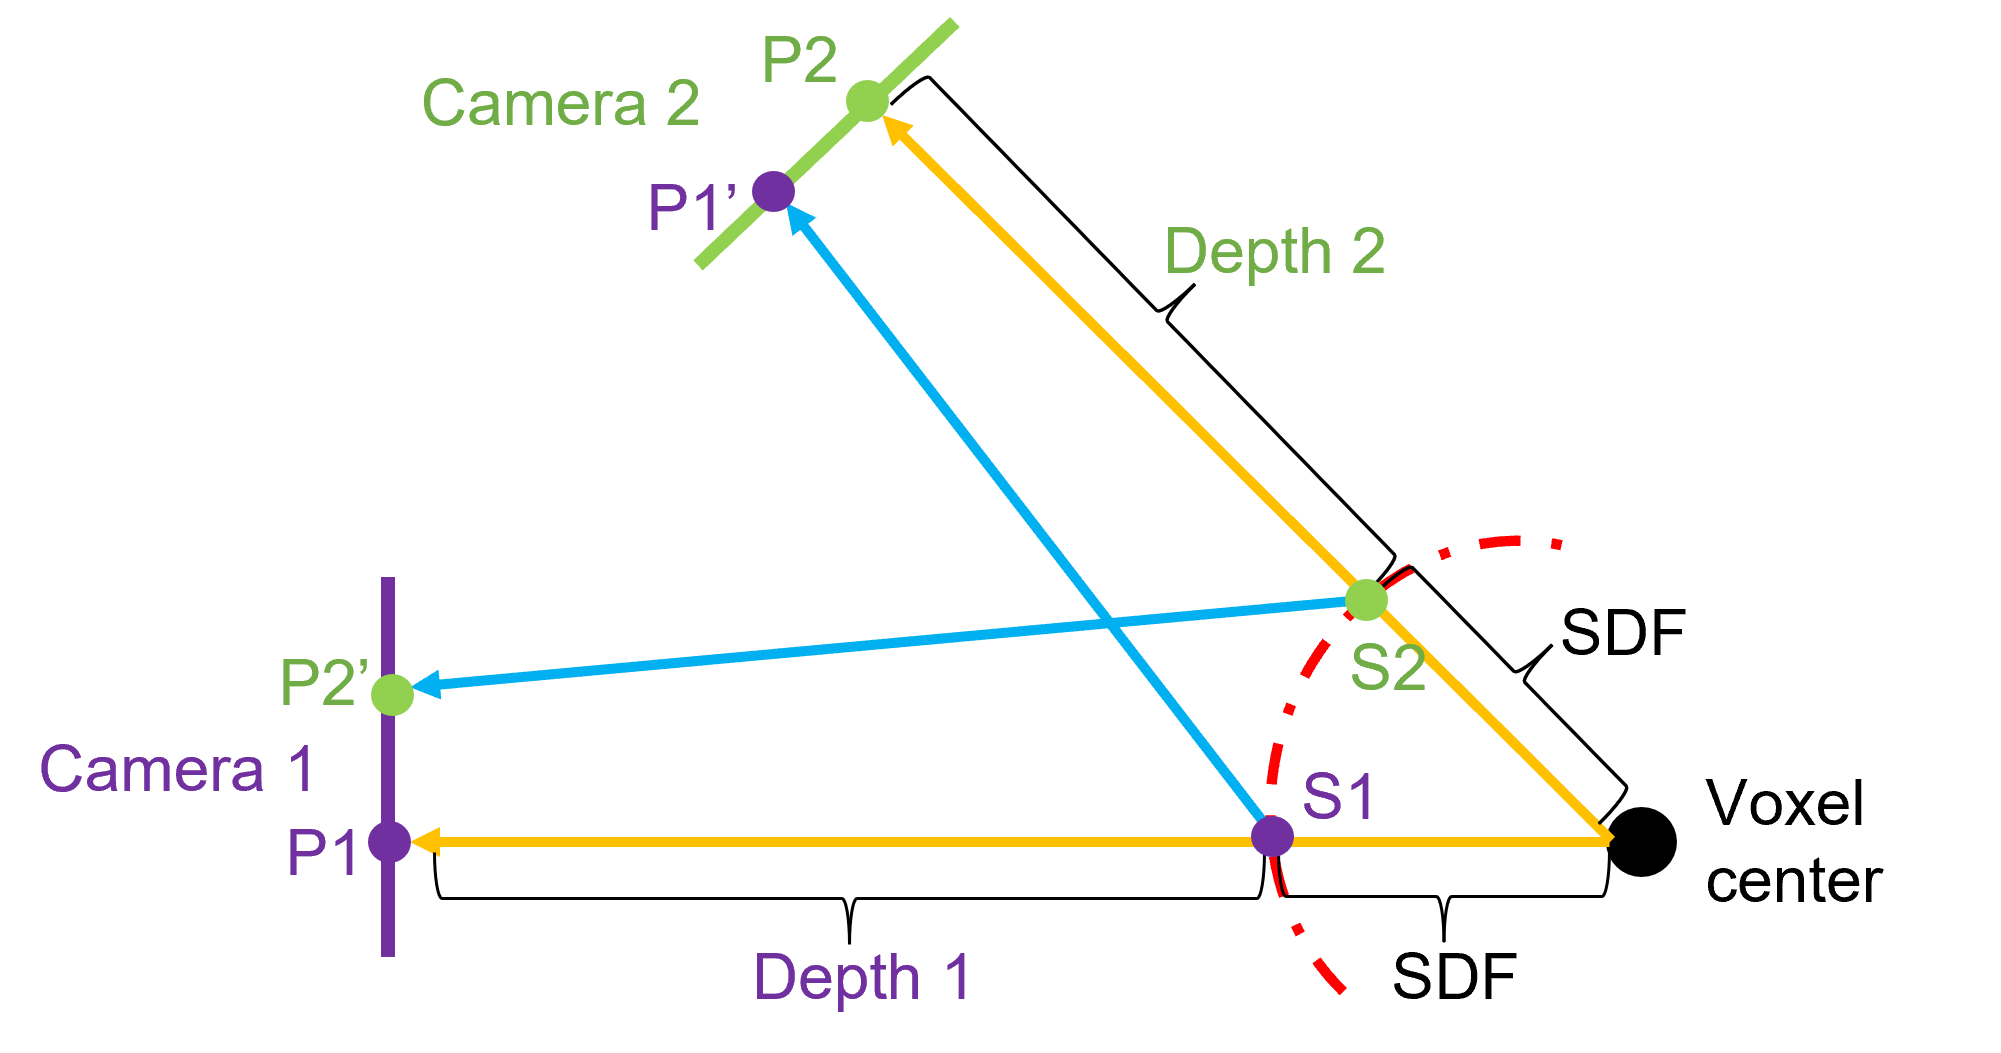
\includegraphics[width=1.0\textwidth]{figures/sdf_loss_a.png}}
\end{minipage}
\hfill
\begin{minipage}{0.51\linewidth}
  \centerline{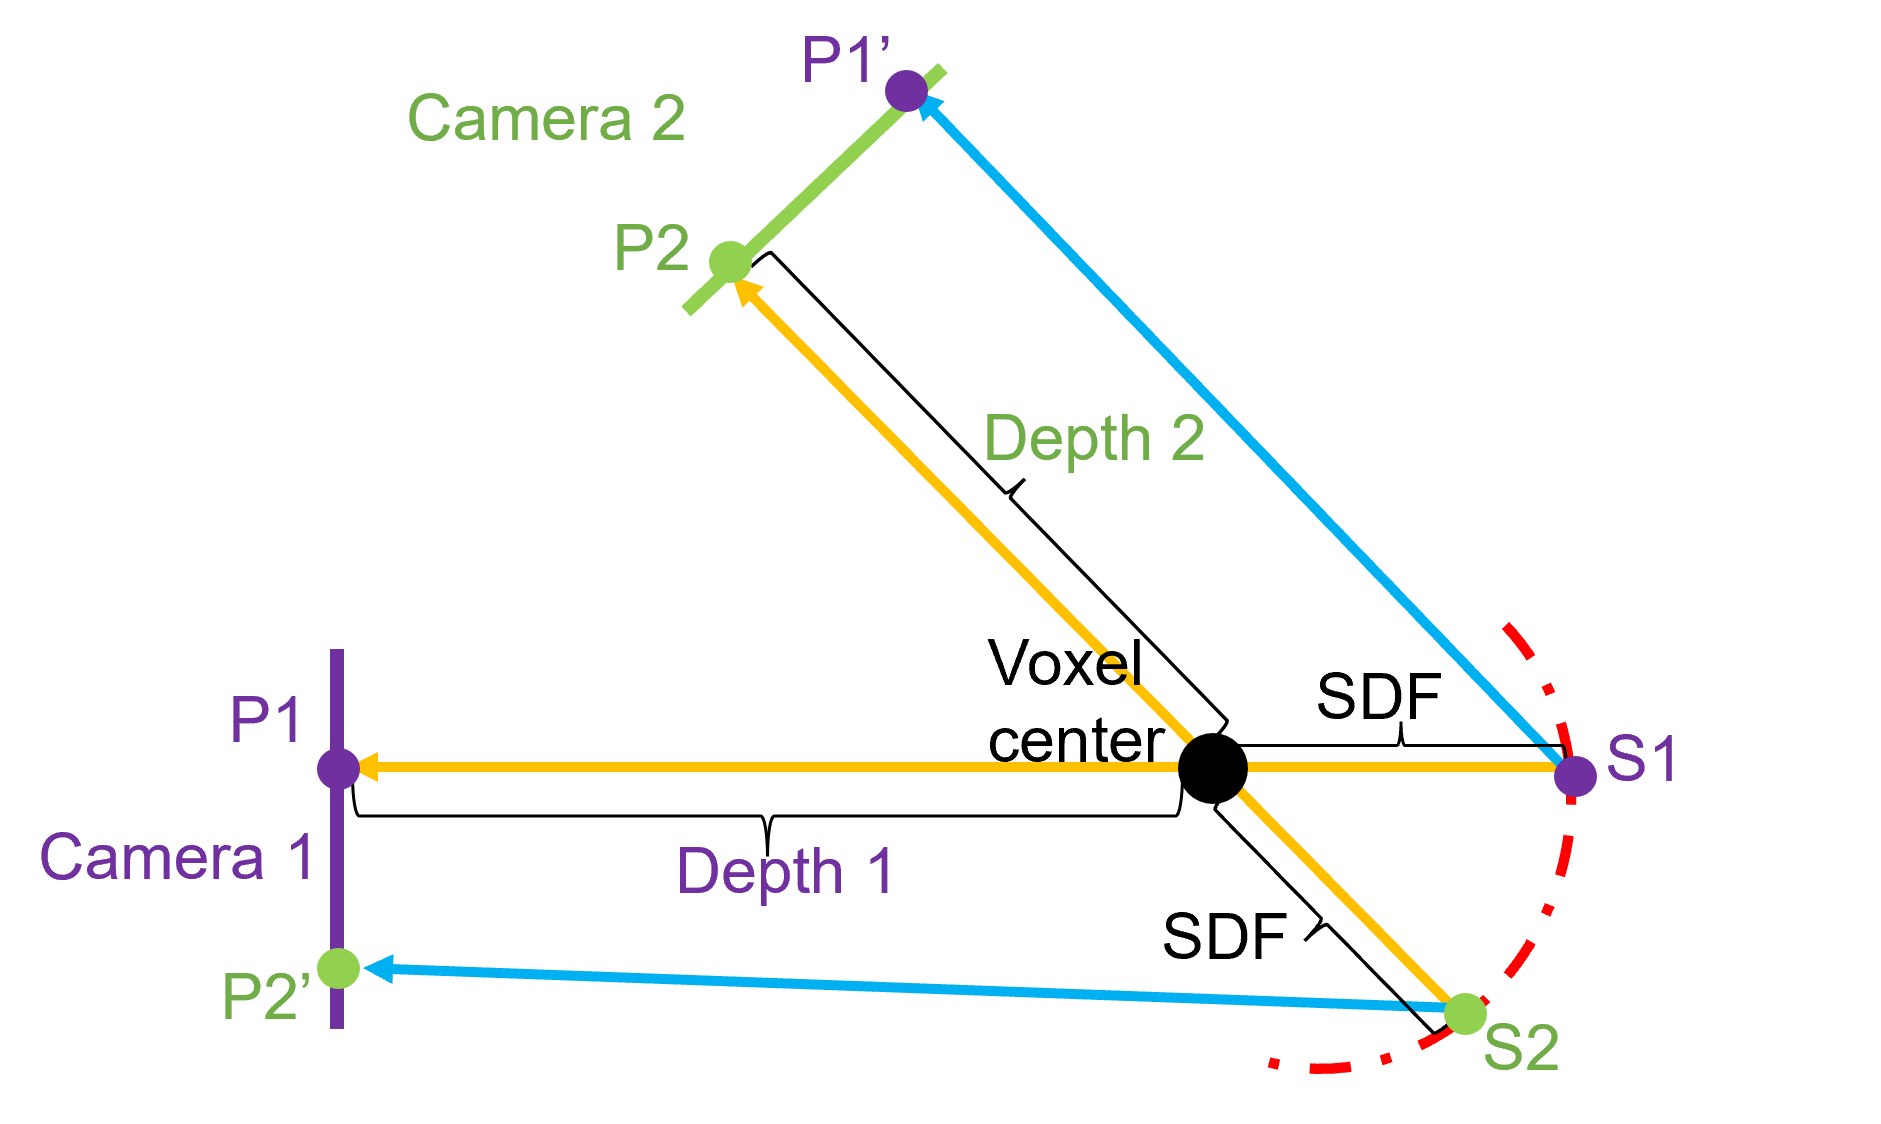
\includegraphics[width=1.0\textwidth]{figures/sdf_loss_b.png}}
\end{minipage}
\vspace{-5mm}
\caption{\textbf{Self-supervised SDF photometric loss between source and target views}. \textbf{Left:} Voxel center is inside of the surface, SDF is negative. Orange arrows show projecting rays from voxel centers to 2D pixels (P1, P2) on each camera plane, blue arrows show reprojection of surface 3D points (S1, S2) to 2D pixels (P1', P2') in each camera plane. Surface points are estimated by SDF estimation. \textbf{Right:} Voxel center is outside of the surface, SDF is positive. \textbf{The loss is extended to all n views in a fragment}.}
\label{fig:sdf photometric loss}
\vspace{-5mm}
\end{figure*}

\vspace{-2mm}
\section{Method}
\label{sec:method}
\vspace{-2mm}
\subsection{MonoSelfRecon Framework}
\quad Figure \ref{fig:pipeline} shows our MonoSelfRecon framework. In both training and testing, we take the input monocular RGB sequence and camera poses, and reconstruct 3D mesh of the whole scene. We select key frames following the process in \cite{key_select}, where we consider a valid frame to be ``greater than 15 degree in rotation or 0.3 meter in translation'' to the previous frame. Every $n$ consecutive key frames form a scene fragment. Fragments are fed as inputs, from which, the network extracts 2D features per key frame, creates 3D feature volume and jointly estimates SDF and NeRF using separate decoders at three pyramid scales. In SDF decoder, 2D features are fused to 3D voxel features and regress to voxel-SDF values at each level with 3D sparse convolution. Every time the network only estimates SDF corresponding to the fragment in a $[N,N,N]$ 3D voxel region, the Gated Recurrent Unit (GRU) module at each level updates SDF, fuses reconstruction from previous fragments, and completes the whole scene. During training, self-supervised losses are implemented between SDF-input, NeRF-input, and SDF-NeRF, with detailed discussion in \ref{sec:losses}. During testing, 3D mesh can be obtained from SDF through marching cube\cite{marchingcube}.  

\noindent
\textbf{Attentional View Fusion}.
For each fragment, 3D voxel features can be simply obtained by projecting the 3D voxel to each 2D view in the fragment, searching for visible corresponding pixels, and averaging 2D features. However, since each view have different distance, angle, and occlusion to voxels, 2D features from different views should not contribute the same to 3D features. Inspired by recent works \cite{vortx}, we use an attentional view fusion module by adding a light transformer before averaging features. The transformer takes unordered sequence of 2D features and updates weighted features before average to 3D, which enables more flexibility to adjust the contribution of each frame to the fragment. Although simple, this module achieves significant improvement as shown in the ablation study in Table \ref{table:scannet_ablation}.

\noindent
\textbf{GRU}. 
We adapt the GRU module from \cite{neucon}. With camera poses, it is simple to concatenate fragments and replace the overlapping voxels of latter fragment to the previous one, but it ignores the effect of the latter views to the previous ones. Once fusing 3D voxel features from 2D and before regressing voxel-SDF at each level, the GRU module takes 3D voxel features of both previous and current fragments as input to update the current features. GRU fusion makes an obvious improvement as shown in the ablation study in Table \ref{table:scannet_ablation}. 


\noindent
\textbf{NeRF.} We adopt the generalizable MPI (MultiPlane-Images)-NeRF \cite{mpi, mpi-nerf, mononerf}, introduce it to the framework and jointly train with SDF to boost SDF estimation. The core idea is to use an explicit encoder on top of standard positional encoding to enable implicit NeRF with generalization ability. The NeRF estimation also further boosts our SDF performance as shown in the ablation study in Table \ref{table:scannet_ablation}.

\subsection{Self-supervised Losses}
\label{sec:losses}

\noindent
\textbf{SDF Photometric Loss}. Figure \ref{fig:sdf photometric loss} shows a simplified version of the loss implementation between two camera views, where the corresponding 2D coordinates (P1 and P2) can be found by tracing rays (orange arrows) to camera planes. SDF is the distance between a point to its nearest surface, where the value is negative when the point is inside of the surface, and positive when it is outside of the surface. The model estimates SDF per voxel. The depth $\hat{D}_{cam}$ can be estimated by Eq. \ref{eq:get_depth}, where $V_{world}$ is 3D world coordinate of the pre-defined voxel center, $T_{world\xrightarrow{}cam}$ is camera extrinsic, $\hat{SDF}$ is the estimated voxel-SDF from the model. With depth and voxel center in the camera coordinate, the surface points S1 and S2 can be estimated by Eq. \ref{eq:get_surface}, where $\vec{ray}$ is the unit vector at ray direction (orange arrows), and $\hat{S}_{cam}$ is the 3D coordinate of a surface point in the camera view. Finally, the reconstructed pixels are obtained by reprojecting (blue arrows) surface points S1, S2 to camera 2 and 1 as Eq. \ref{eq:point_proj}, where K is camera intrinsic, $T_{cam\xrightarrow{}cam'}$ is camera pose from cam to cam'. P-P' is a pixel reconstruction pair with same photometric intensity, where a photometric consistency loss can be derived as Eq. \ref{eq:pts_loss}. The exact pixel intensities $I_{cam}(P)$ and $I_{cam'}(P')$ are obtained with bilinear interpolation from projected 2D points lying between integer coordinates, and the loss is only traced to the points lying within the camera planes.
\vspace{-3mm}
\begin{equation}
\begin{split}
    V_{cam} = T_{world\xrightarrow{}cam}V_{world} \\
    \hat{D}_{cam} = V_{cam} + \hat{SDF}
    \label{eq:get_depth}
\end{split}
\end{equation}
\vspace{-6mm}

\vspace{-5mm}
\begin{equation}
\begin{split}
    \hat{S}_{cam}(x, y, z) = V_{cam}(x, y, z) + |\hat{SDF}| \Vec{ray}(x, y, z)
    \label{eq:get_surface}
\end{split}
\end{equation}
\vspace{-6mm}

\vspace{-5mm}
\begin{equation}
\begin{split}
    P = Interp(KV_{cam}) \\
    P' = Interp(K'T_{cam\xrightarrow{}cam'}\hat{S}_{cam})
\end{split}
\label{eq:point_proj}
\end{equation}
\vspace{-6mm}

\vspace{-4mm}
\begin{equation}
    L_{sdf} = \sum_{P \in cam}\sum_{P'\in cam'}{|(I_{cam}(P) - I_{cam'}(P')|}
\label{eq:pts_loss}
\end{equation}
\vspace{-4mm}

\iffalse
We make an assumption to set up this point-wise self-supervised SDF loss. Although the distance from the voxel center to different surface points varies - only the nearest distance is SDF. Since the network estimates one SDF value per voxel, we use the same estimated SDF value corresponding to the same voxel center to estimate surface points for different camera views. However, previous supervised works made the same assumption to implement TSDF fusion  \cite{atlas, neucon} and get TSDF ground truth from the depth map. More specifically, instead of using the nearest distance, they take the average distances from all views. Similarly, we assign this task to the network, when the resolution is large enough (voxel size is small enough), the network is trained to get to the average distance that optimizes the consistency loss between all camera views.
\fi

In practice, we implement the loss across all views in the scene fragment and take the weighted average loss, where the weight is in direct proportion to the number of the candidate P-P' pair. If P' lies outside of the other camera's plane, we ignore this P-P' pair. For SFM-based self-supervised depth works, they start from 2D pixel and ends up at 2D pixel to jointly regress depth and camera pose. However, we start from 3D voxel center and end up at 2D pixel to only regress the depth model while taking camera pose as prior, which is why SFM-based self-supervised depth estimation has scale ambiguity, while our SDF estimation is directly in real scale. 

\noindent
\textbf{SDF Co-Planar Loss}. Photometric constraints are insufficient for indoors scenes due to large non-textured regions and in-plane rotations. Thus, we take advantage of the special geometric constraints in indoor scenes. Most indoor scenes have large planes such as walls, floors, and ceilings, where textures within such planes are mostly similar. Inspired by \cite{p2net, planercnn, planenet, piece-wise} that implement planar constraints in 2D depth maps, we extend it to 3D SDF. Specifically, we adopted `Felzenszwalb superpixel segmentation' \cite{plane_seg} to extract `super-pixels', which covers piece-wise large group of regions that have low pixel intensity gradients, which are considered as a planar region. The algorithm uses greedy search to extract super-pixels and is free of learning. Based on the planar segmentation and the depth planar constraints from \cite{structdepth}, we propose a voxel-SDF driven co-planar loss.

Our goal is to derive plane parameters under planar constraints, and learn the plane parameters in a self-supervised manner. Specifically, the plane segmentation extracts $n$ super-pixels from a 2D image, with each super-pixel corresponding to a continuous plane. For the 2D projected voxel center point P (as shown in Figure \ref{fig:sdf photometric loss}), if it belongs to super-pixel $SP_m$ in the 2D plane, then the surface 3D point $S$ corresponding to $P$ also belongs to the surface plane of class $m$ in 3D space. Using the surface point $S$, the plane $m$ can be defined as Eq. \ref{eq:plane_onepoint}, where $\hat{s}_{0}$ is an estimated surface point in the plane, and $A_m$ is the plane parameter.

\vspace{-3mm}
\begin{equation}
    A_{m}^T \hat{s}_{0} = 1
    \label{eq:plane_onepoint}
\end{equation}
\vspace{-5mm}

While using only one 3D point to simulate a plane is ill-posed, a large number of estimated 3D surface points are obtained by projecting voxel centers to different camera views. With $n$ 2D projected points $p_1$, $p_2$ ...... $p_n$ belonging to super-pixel $SP_m$, there are $n$ 3D surface points $s_1$, $s_2$, ......, $s_n$ belonging to 3D surface plane $m$. Eq. \ref{eq:plane_onepoint} is extended to Eq. \ref{eq:plane_npoint}, where $\hat{S}_{n} = [\hat{s}_{1}, \hat{s}_{2}, ......, \hat{s}_{n}]$, and $Y_m = \Vec{1} = [1,1,...,1]$.

\vspace{-3mm}
\begin{equation}
    \hat{S}_{n} A_{m}^T  = Y_{m}
    \label{eq:plane_npoint}
\end{equation}
\vspace{-5mm}

The plane parameter $A_{m}$ is then estimated by least-square method as Eq. \ref{eq:least_square}, where $\epsilon$ is a small scalar for stability, and $I$ is an identity matrix.

\vspace{-3mm}
\begin{equation}
    A_m = (\hat{S}_n^T\hat{S}_n+\epsilon I)^{-1}\hat{S}_n^TY_m
    \label{eq:least_square}
\end{equation}
\vspace{-5mm}

With the estimated plane parameter, the pseudo surface points can be retrieve  by $\hat{S_n}' = (A_m^T \hat{S_n})^{-1}$. The pseudo surface and estimated surface are expected to align together, and we implement such a co-planar geometric constraint as the self-supervised co-planar SDF loss as Eq. \ref{eq:plane_loss}.

\vspace{-3mm}
\begin{equation}
    L_{plane} = \sum_{M}\sum_{N}{|\hat{S_n}-\hat{S_n}'|}
\label{eq:plane_loss}
\end{equation}
\vspace{-3mm}

\noindent
\textbf{Depth Consistency Loss.} We also propose depth consistency loss to further boost SDF from NeRF. Specifically, we estimate sparse Pseudo-SDF depth for target views from estimated SDF (as Figure \ref{fig:sdf photometric loss}), and render NeRF-depth for corresponding target views. Since Pseudo-SDF depth is in real scale, we first use it to recover NeRF-depth's scale, and enforce consistency between the two estimated depths. 

\vspace{-3mm}
\begin{equation}
    L_{depth} = \sum_{N}\sum_{D \in cam}{|\hat{D_{sdf}}-\hat{D_{NeRF}}|}
\label{eq:depth_loss}
\end{equation}
\vspace{-3mm}

\noindent
where $\hat{D_{sdf}}$ and $\hat{D_{NeRF}}$ are Pseudo-SDF depth and the scale-recoverd NeRF-depth, respectively.

\noindent
\textbf{Total Loss.} We implement standard NeRF losses for NeRF encoder, including RGB consistency with input images, SSIM, and smooth loss, and we jointly train everything end-to-end in pure self-supervision.

\vspace{-8mm}
\begin{equation}
    L_{NeRF} = L_{rgb} + L_{smooth} + (1 - SSIM)
\label{eq:nerf_loss}
\end{equation}
\vspace{-6mm}

\noindent
The total loss is the weighted sum of all losses, where $\lambda$s are the weights,

\vspace{-3mm}
\begin{multline}
    L_{total} = \lambda_{sdf}L_{sdf} + \lambda_{plane}L_{plane} \\ + 
    \lambda_{depth}L_{depth} + \lambda_{NeRF}L_{NeRF}
\label{eq:total_loss}
\end{multline}
\vspace{-5mm}
\section{Experiments}
\subsection{Experiment Setup}
For all the experiments, we run the algorithm with one single GPU (NVIDIA Tesla V100) and CPU (Intel Xeon E5-2680). 
Following ~\citet{peng2021amp}, we use the average pose error as the main metric. The average pose error over the whole trajectory of length $T$ with $J$ joints is computed between the pose of the simulated character and the reference motion using the relative positions of each joint with respect to the root joint (in units of meters):
\begin{equation}
\small
    e = \frac{1}{T} \sum_{t\in T} \frac{1}{\lVert J \rVert} \sum_{j \in J} \lVert (p^j_t - p_t^{root}) - (\hat{p}^j_t - \hat{p}_t^{root}) \rVert_2, 
\end{equation}
where $p^j_t$ and $\hat{p}^j_t$ are the position of $j$-th joint of the simulated motion and reference motion at timestamp $t$ in the 3D cartesian space and $root$ refers to the root joint. 
We mainly compare with DeepMimic~\citep{peng2018deepmimic}, Spacetime Bound~\citep{ma2021learning}, and Adversarial Motion Prior (AMP)~\citep{peng2021amp}. Dynamic Time Warping~\citep{sakoe1978dynamic} is applied to synchronize the simulated motion and the reference motion following the convention.

\textbf{Cyclic Motions.} Besides mimicking a single motion clip, a popular benchmark for motion mimicking is to imitate cyclic motions like walking and running, where a single cycle of the motion is provided as the reference motion and the character learns to repeat the motion for 20 seconds. 
Typically, a curriculum is designed to gradually increase the maximum rollout episode to 20 seconds during training~\citep{yang2021efficient, peng2018deepmimic}. In our experiment, we remove all bells and whistles and fix the maximum rollout episode to 4 seconds during the training. DiffMimic can produce a 20-second long cyclic rollout even though it only sees 4-second rollouts in training. {The motion clips are directly borrowed from AMP~\citep{peng2021amp}, which are originally collected from a combination of public mocap libraries, custom recorded mocap clips, and artist-authored keyframe animations.}


\begin{table}[]
    \centering
    \begin{tabular}{cccc}
         \hspace{-10pt}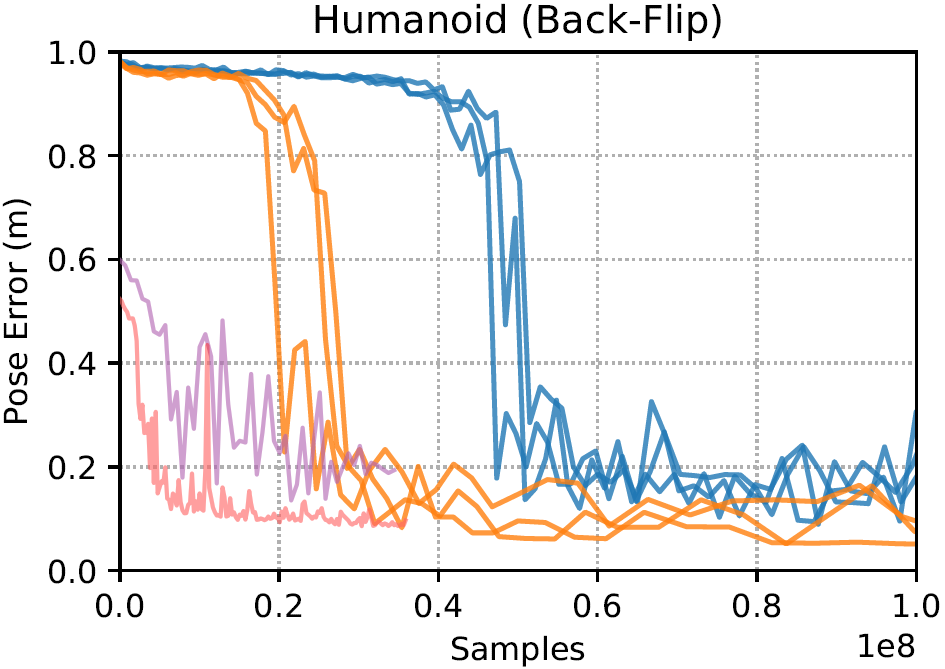
\includegraphics[width=0.23\textwidth]{figures/mixed_backflip.png}
         &
         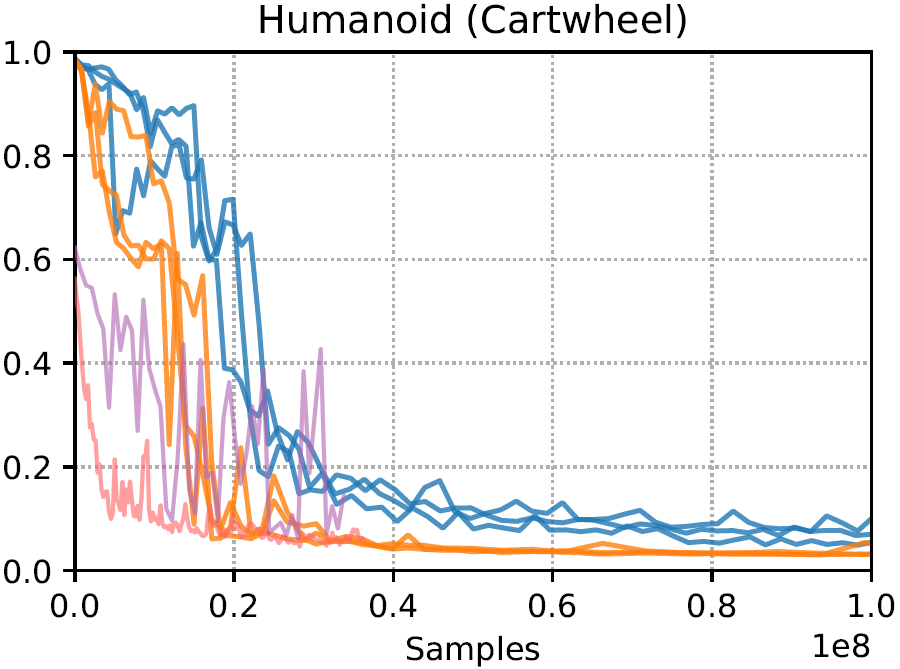
\includegraphics[width=0.23\textwidth]{figures/mixed_cartwheel.png}
         &
         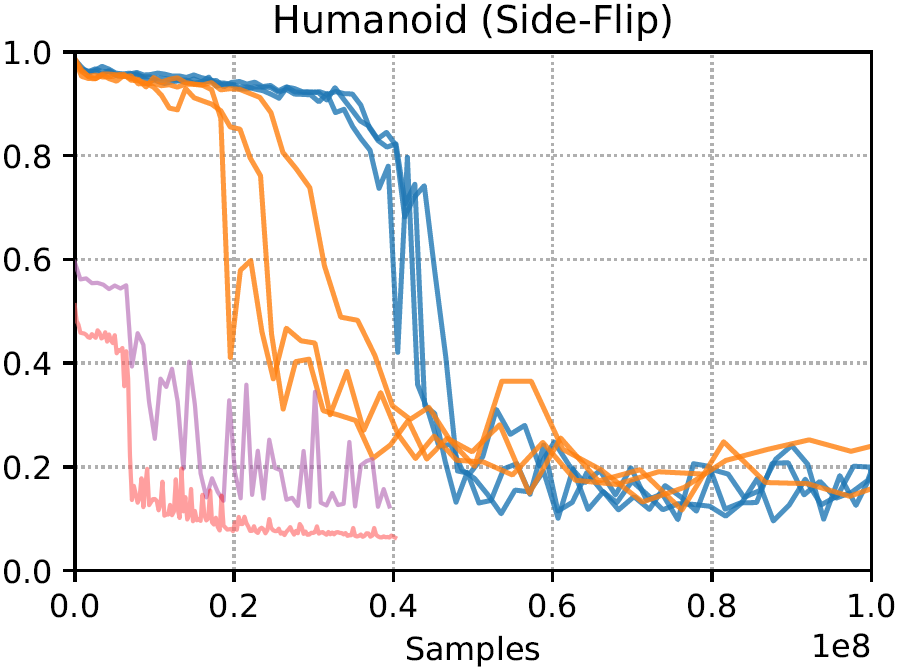
\includegraphics[width=0.23\textwidth]{figures/mixed_sideflip.png}
         &
         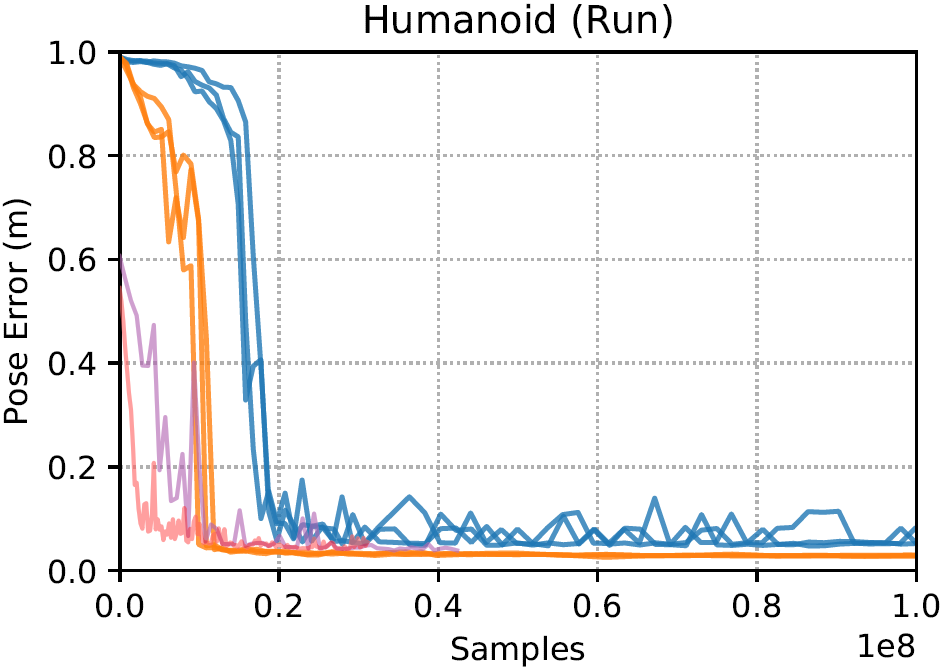
\includegraphics[width=0.23\textwidth]{figures/mixed_run.png}
         \\
         \hspace{-10pt}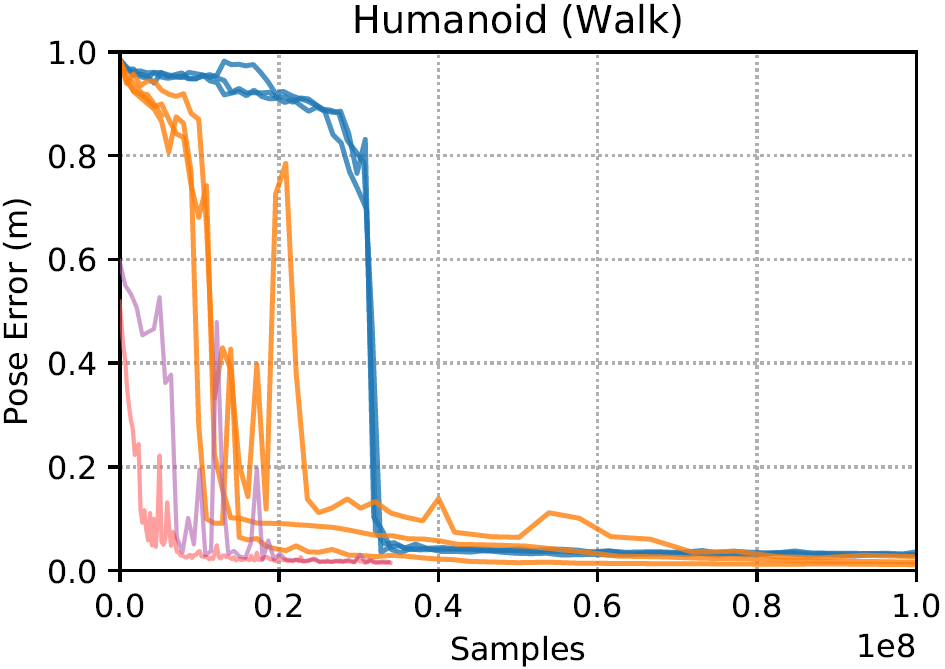
\includegraphics[width=0.23\textwidth]{figures/mixed_walk.png}
         &
         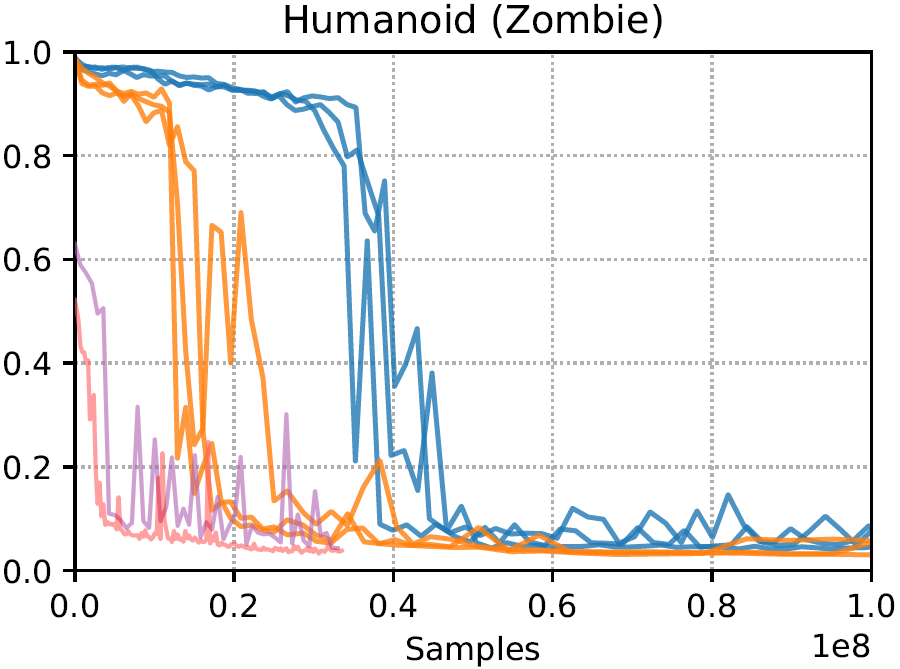
\includegraphics[width=0.23\textwidth]{figures/mixed_zombie.png}
         &
         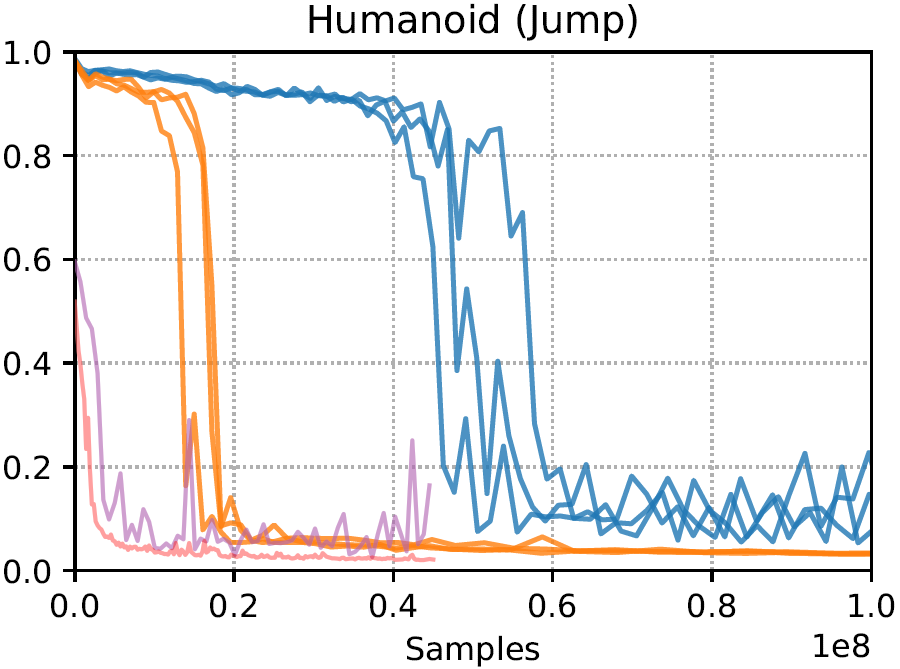
\includegraphics[width=0.23\textwidth]{figures/mixed_jump.png}
         &
         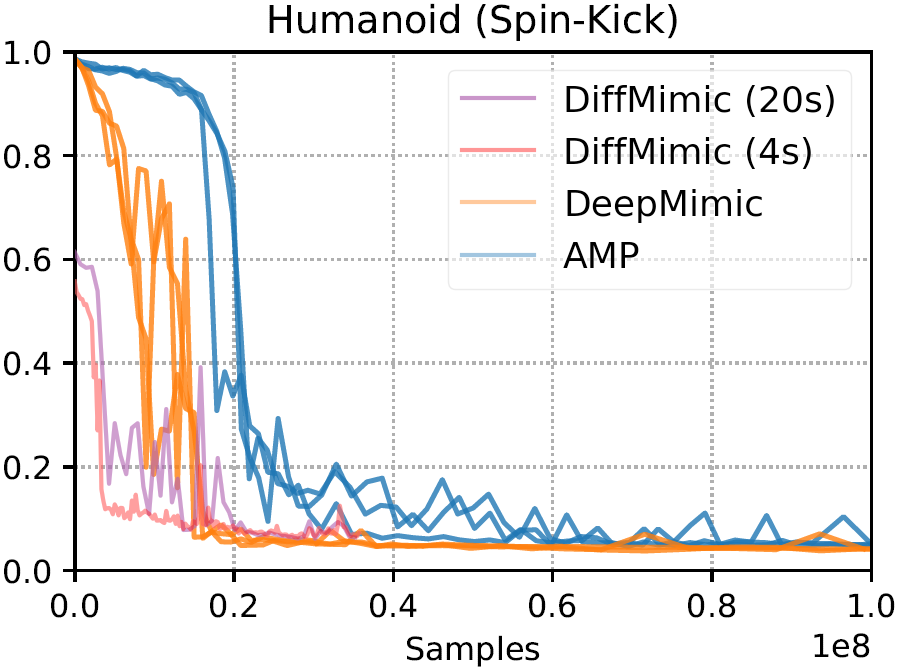
\includegraphics[width=0.23\textwidth]{figures/mixed_spinkick_legend.png}
    \end{tabular}
    \captionof{figure}{Pose error versus the number of samples. DiffMimic (4s): rollout 4 seconds of Diffmimic for evaluation.  DiffMimic (20s): rollout 20 seconds of Diffmimic for evaluation. In general, DiffMimic allows the policy to generate high-quality motions with less than $3.5 \times 10^7$ samples.  
    We refer the readers for more results to the appendix.}
    \label{fig:imitate_one}
\end{table}

\subsection{Comparison on Motion Mimicking}
In this section, we aim to understand 1) efficiency; 2) the quality of the learned policy of DiffMimic. Following the conventions of previous works~\citep{peng2018deepmimic, peng2021amp, ma2021learning}, we count the number of samples required to train the policy to rollout for 20 seconds without falling. The pose error is calculated over the horizon of 20 seconds.

\textbf{Analytical gradients enhance the sample efficiency in motion mimicking.} We show the comparison between DiffMimic, DeepMimic, and Spacetime Bound on sample efficiency in Table~\ref{sampleeff}. DeepMimic is an RL-based algorithm with a careful reward design. Spacetime Bound performs hyperparameter searching for DeepMimic to further enhance the sample efficiency. Our results show that DiffMimic constantly outperforms DeepMimic in terms of sample efficiency. The analytical gradients provided by the differentiable simulation allow us to compute policy gradient with a small number of samples while the RL-based algorithm requires a large batch to have a decent estimate. Compared with Spacetime Bound, DiffMimic is much more stable and consistent over various tasks. We notice that Spacetime Bound may require more samples than DeepMimic even for simple tasks like \textit{Jump}. We show the learning curve of DiffMimic over eight different tasks in Fig.~\ref{fig:imitate_one}. It shows that DiffMimic generally learns high-quality motions (pose error $<$ 0.15) with less than 2e7 samples, even for challenging tasks like \textit{Backflip}. In terms of the wallclock time, DiffMimic learns to perform \textit{Backflip} in 10 minutes and learns to cycle it in 3 hours ($14.88 \times 10^6$ samples), which can be found in our qualitative results.
\begin{wrapfigure}[16]{r}{0.38\columnwidth}
     \centering
     \vspace{-10pt}
         \centering
         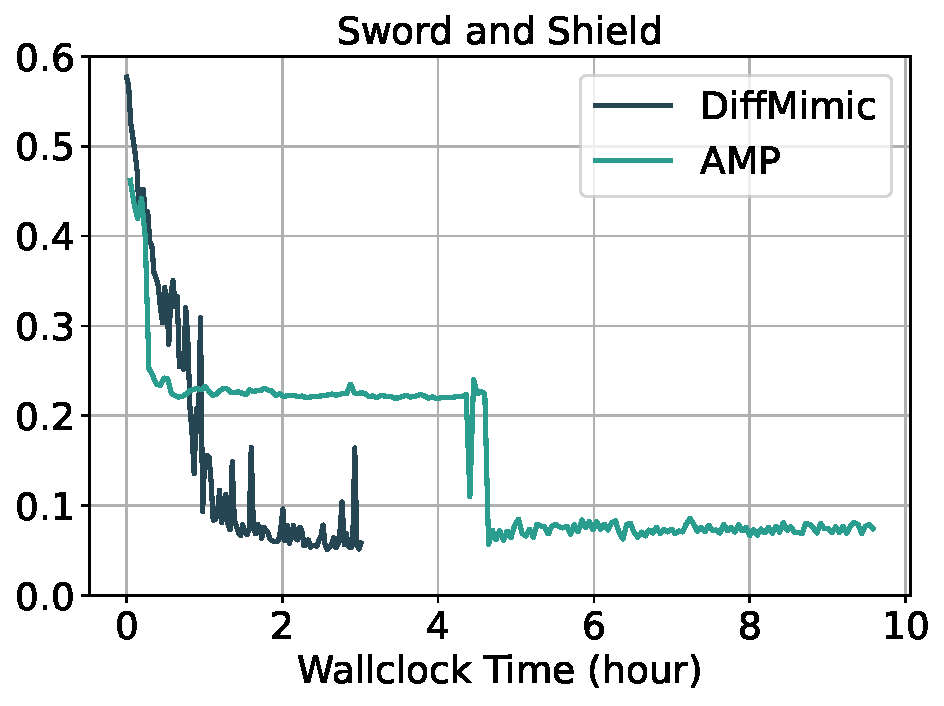
\includegraphics[width=0.38\textwidth]{figures/wallclock_sword.pdf}
     \caption{Wallclock training time versus pose error for DiffMimic and AMP. DiffMimic takes half of the training time required by AMP to have a comparable result.}
    \label{fig:Wallclock time}
\end{wrapfigure}

\textbf{DiffMimic can learn high-quality motions.} The average pose error for 12 different motion tasks is shown in Table~\ref{poseerror}. DiffMimic outperforms AMP consistently and has comparable performance to DeepMimic. 
Noticeably, DiffMimic only needs to see the demonstrations of 4 seconds to achieve a similar performance of DeepMimic with 20 seconds cyclic rollout, which indicates stable and faithful recovery of the reference motion. This further corroborates the efficacy of DiffMimic. 

\textbf{Analytical gradients accelerate the learning speed in motion mimicking.} As it generally takes more time to compute analytical gradients than the estimated one, it is natural to compare the wall-clock time for each algorithm. Since the implementation of DeepMimic does not utilize GPU for parallelization, we choose to compare DiffMimic with AMP. The implementation of AMP utilizes the highly parallelized environment, IsaacGym~\citep{makoviychuk2021isaac}. Both approaches do not require manual reward design and utilize GPU for acceleration. We compare DiffMimic and AMP on a task where a humanoid character is wielding a sword and a shield to perform a 3.2-second attack move (shown in Appendix Fig.~\ref{fig:sword}). The hyperparameter of AMP is from its official release of code.
We show the comparison with respect to wallclock time in Fig.~\ref{fig:Wallclock time}. %
DiffMimic takes half of the training time required by AMP to have a comparable result.



\begin{table}[t]
\caption{Pose error comparison in meters.  $\textrm{T}_\textrm{cycle}$ is the length of the reference motion for a single cycle. The error is averaged on 32 rollout episodes with a maximum length of 20 seconds.}
\fontsize{8.8}{9}\selectfont
\begin{center}
\begin{tabular}{lcccc}
\toprule
Motion & $\textrm{T}_\textrm{cycle}$(s) &  DeepMimic & AMP & Ours\\
\midrule
Back-Flip & 1.75 & 0.076 $\pm$ 0.021 & 0.150 $\pm$ 0.028 & 0.097 $\pm$ 0.001 \\
Cartwheel & 2.72 & 0.039 $\pm$ 0.011 & 0.067 $\pm$ 0.014 & 0.040 $\pm$ 0.007 \\
Crawl & 2.93 & 0.044 $\pm$ 0.001 & 0.049 $\pm$ 0.007 & 0.037 $\pm$ 0.001 \\
Dance & 1.62 & 0.038 $\pm$ 0.001 & 0.055 $\pm$ 0.015 & 0.070 $\pm$ 0.003 \\
Jog & 0.83 & 0.029 $\pm$ 0.001 & 0.056 $\pm$ 0.001 & 0.031 $\pm$ 0.002 \\
Jump & 1.77 & 0.033 $\pm$ 0.001 & 0.083 $\pm$ 0.022 & 0.025 $\pm$ 0.000 \\
Roll & 2.02 & 0.072 $\pm$ 0.018 & 0.088 $\pm$ 0.008 & 0.061 $\pm$ 0.007 \\
Run & 0.80 & 0.028 $\pm$ 0.002 & 0.075 $\pm$ 0.015 & 0.039 $\pm$ 0.000 \\
Side-Flip & 2.44 & 0.191 $\pm$ 0.043 & 0.124 $\pm$ 0.012 & 0.069 $\pm$ 0.001\\
Spin-Kick & 1.28 & 0.042 $\pm$ 0.001 & 0.058 $\pm$ 0.012 & 0.056 $\pm$ 0.000\\
Walk & 1.30 & 0.018 $\pm$ 0.005 & 0.030 $\pm$ 0.001 &  0.017 $\pm$ 0.000 \\
Zombie & 1.68 & 0.049 $\pm$ 0.013 & 0.058 $\pm$ 0.014 & 0.037 $\pm$ 0.002 \\
\bottomrule
\end{tabular}
\label{poseerror}
\end{center}
\end{table}



\begin{table}[t]
\caption{Number of samples required to roll out 20 seconds without falling in $(10^6)$. {Percentage: change in the fraction of the DeepMimic samples.}}
\begin{center}
\begin{tabular}{lcr|r|r}
\toprule
Motion & $\textrm{T}_\textrm{cycle}$(s) &  DeepMimic  & Spacetime Bound  & Ours\\
\midrule
Back-Flip & 1.75 & 31.18 & 41.20 \plusstyle{+32.1\%} & 14.88 \minusstyle{-52.2\%} \\
Cartwheel & 2.72  & 30.45 & 17.35 \minusstyle{-43.0\%} & 13.92 \minusstyle{-54.2\%}\\
Walk & 1.25  & 23.80 & 4.08 \minusstyle{-79.5\%} & 7.92 \minusstyle{-66.7\%} \\
Run & 0.80  & 19.31 & 4.11 \minusstyle{-78.7\%} & 8.16 \minusstyle{-57.7\%} \\
Jump & 1.77  & 25.65 & 41.63 \plusstyle{+77.8\%} & 5.28 \minusstyle{-79.4\%} \\
Dance & 1.62  & 24.59 & 10.00 \minusstyle{-59.3\%} & 16.56 \minusstyle{-32.6\%} \\
\bottomrule
\label{sampleeff}
\end{tabular}
\end{center}
\end{table}



\subsection{Ablation on Truncation length}

Training the policy with DPS would suffer from the vanishing/exploding gradients and local optimal. Recent research~\citep{xu2022accelerated} points out that such a problem can be mitigated by a truncated learning window, which splits the entire trajectory into segments with shorter horizons. we carried out experiments to validate whether such an idea can be directly applied in motion mimicking with DPS. Truncation length refers to the horizon over which the gradient is calculated. The quantitative results are shown in Fig.~\ref{tab:ablation}. Indeed, it is difficult to learn a good policy by propagating the gradient through a whole trajectory that is long. In addition, simply splitting the whole trajectory into segments would worsen the final performance. We hypothesize the naive truncation of the trajectory creates discontinuities in the whole trajectory whereas motions in the trajectory are highly interdependent. For example, how to flip in mid-air closely relates to how the character jumps. We see this as a strong call for a better strategy to handle these two challenges in motion mimicking with DPS.
\subsection{Ablation on Demonstration Replay}

\begin{table}[t]
    \centering
    \vspace{-10pt}
    \begin{tabular}{cccc}
      \hspace{-10pt}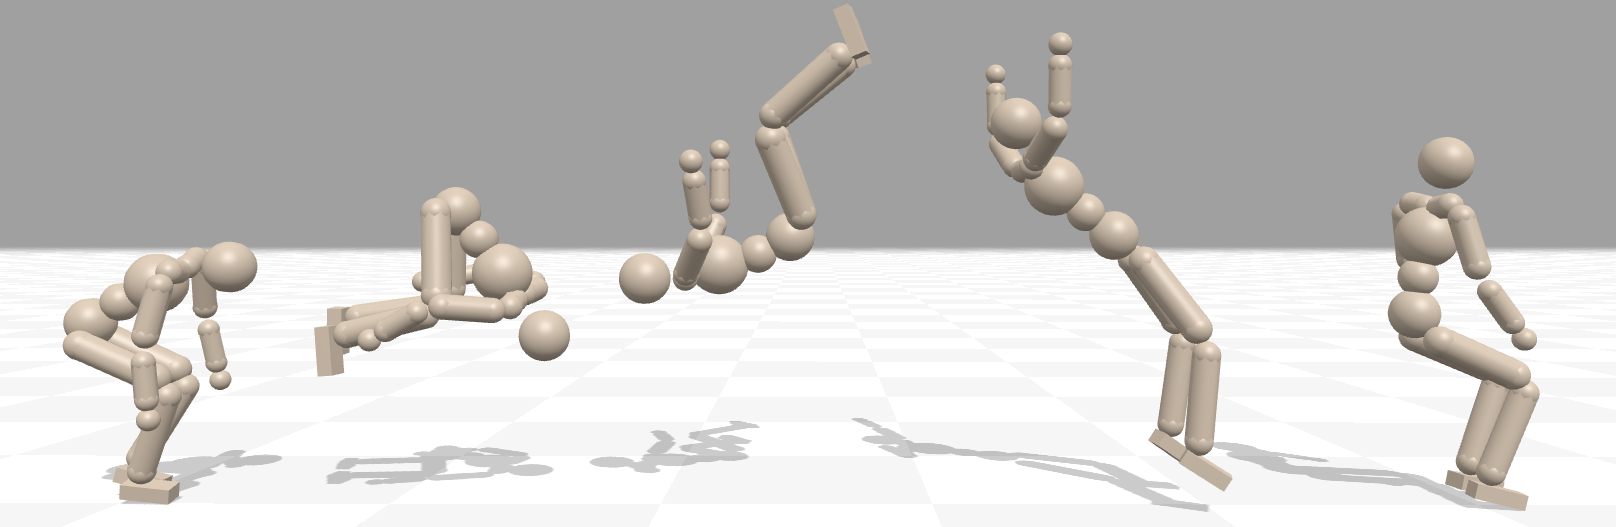
\includegraphics[width=0.4\textwidth]{figures/qp/backflip_demo.png}
      &  
      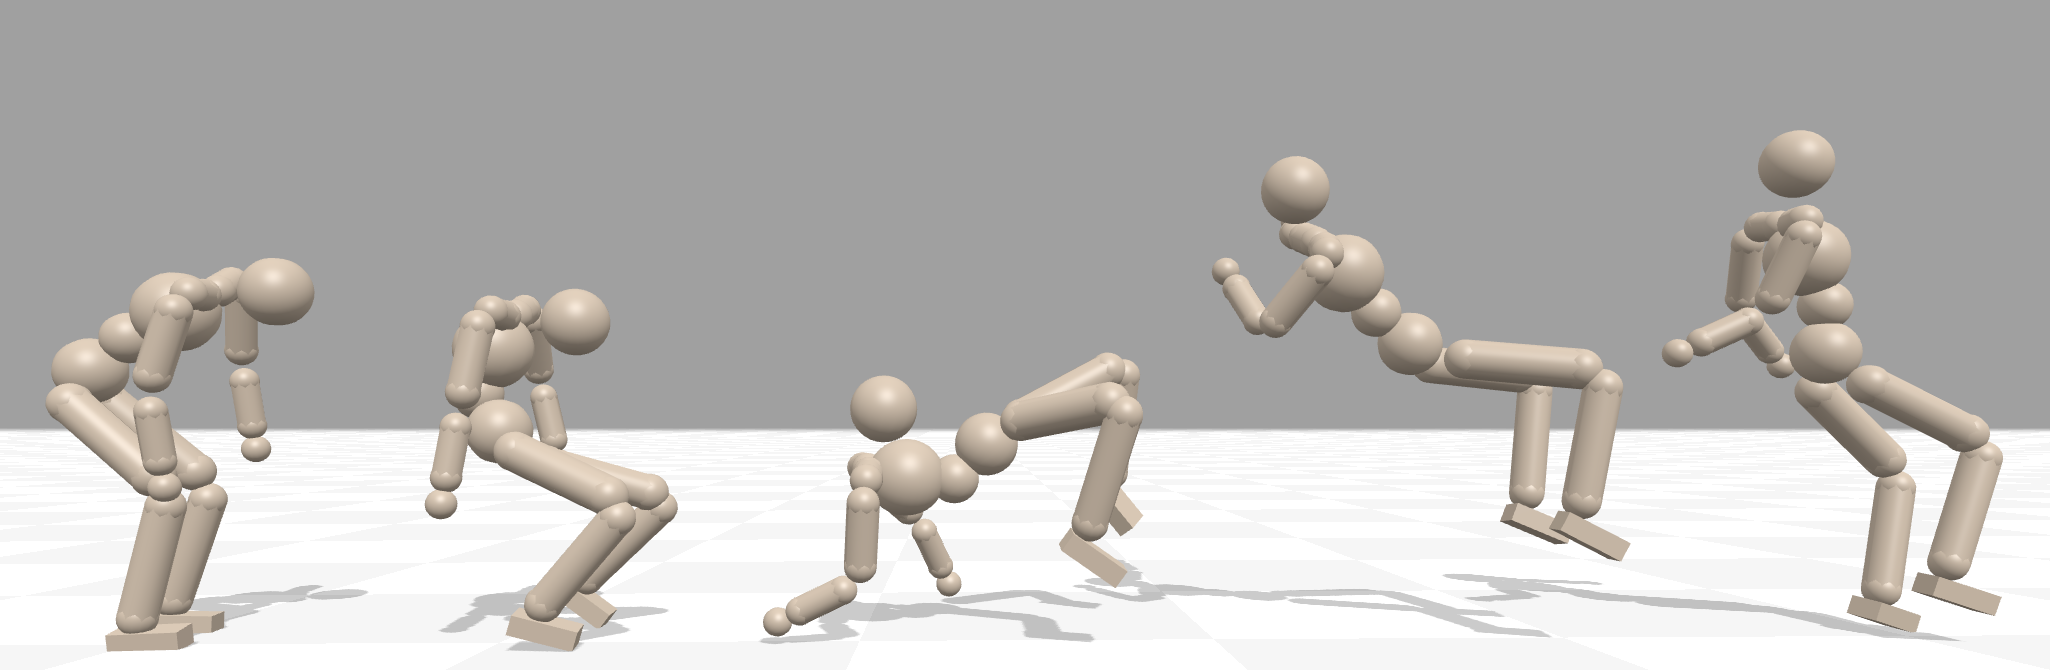
\includegraphics[width=0.4\textwidth]{figures/qp/backflip_trunc1000.png}
        \\
         (a) Reference motion.
         &
         (b) Full Horizon Gradient.
        \\
     \hspace{-10pt}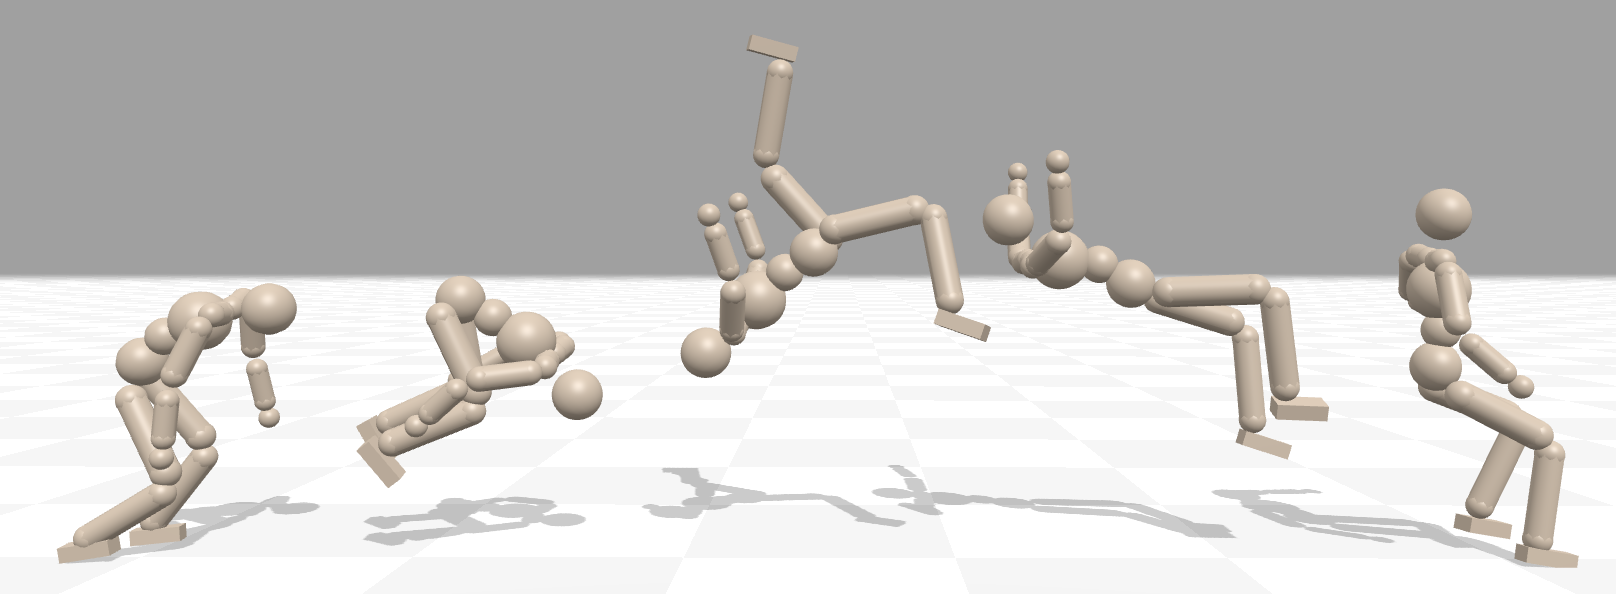
\includegraphics[width=0.4\textwidth]{figures/qp/backflip_random.png}
      &  
      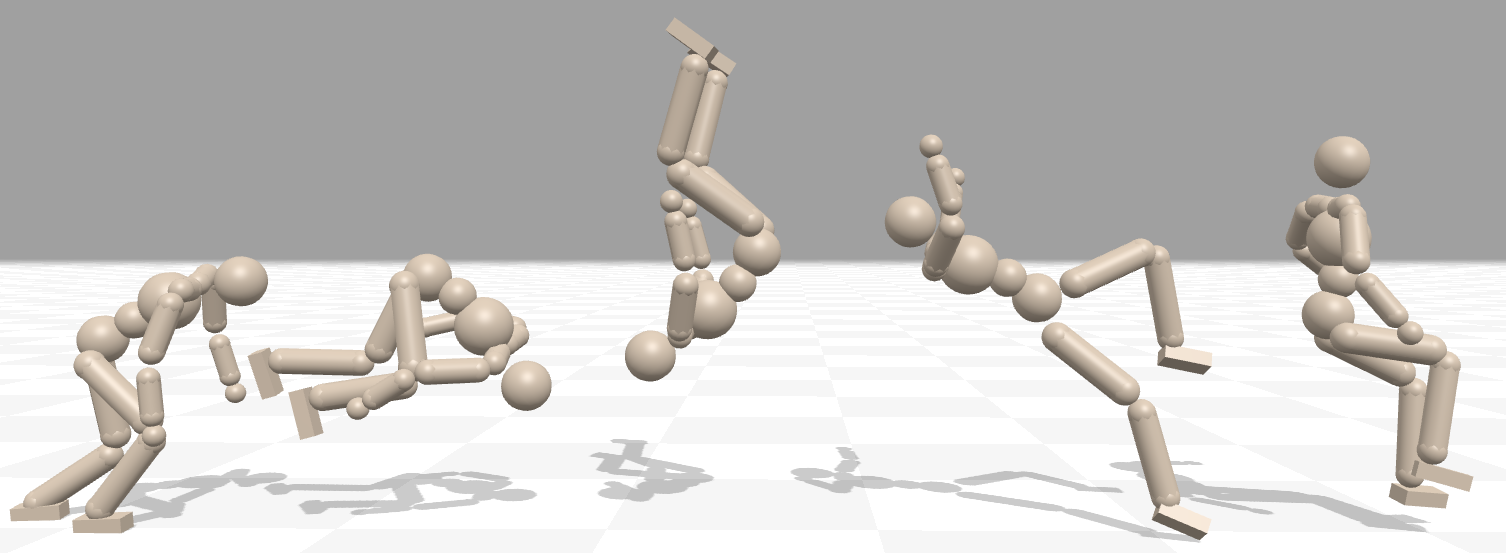
\includegraphics[width=0.4\textwidth]{figures/qp/backflip_err0.4.png}
        \\
        (c) Demonstration Replay (Random).
         &
        (d) Demonstration Replay (Threshold).
    \end{tabular}
    \captionof{figure}{Qualitative results of three variants of DiffMimic with respect to demonstration replay. The policy trained with full horizon gradient fails to jump up. The policy trained with Demonstration Replay (Random) fails to recover the reference motion faithfully. }
    \label{fig:vis_ablation}
\end{table}





\begin{table}[]
    \centering
    \begin{tabular}{ccc}
    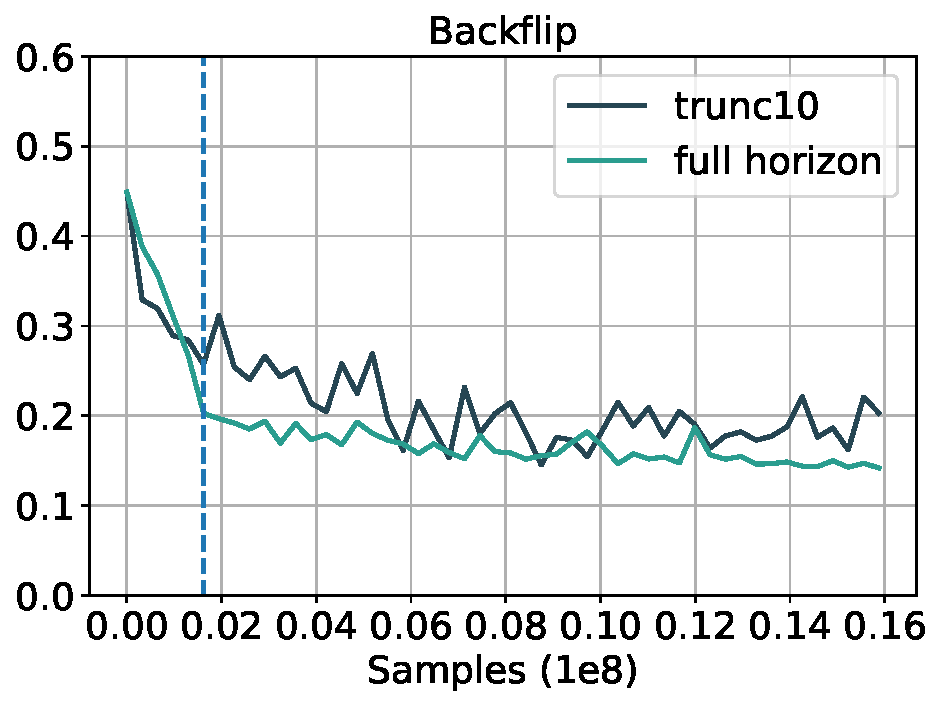
\includegraphics[width=0.3\textwidth]{figures/trunc_backflip.pdf}&
    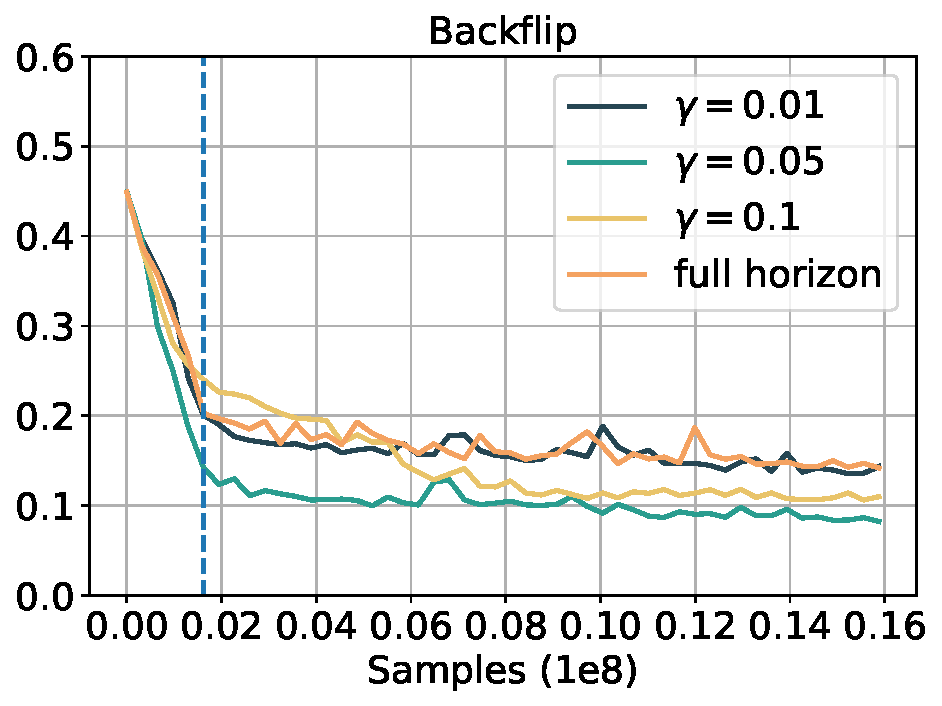
\includegraphics[width=0.3\textwidth]{figures/rand_backflip.pdf}&
    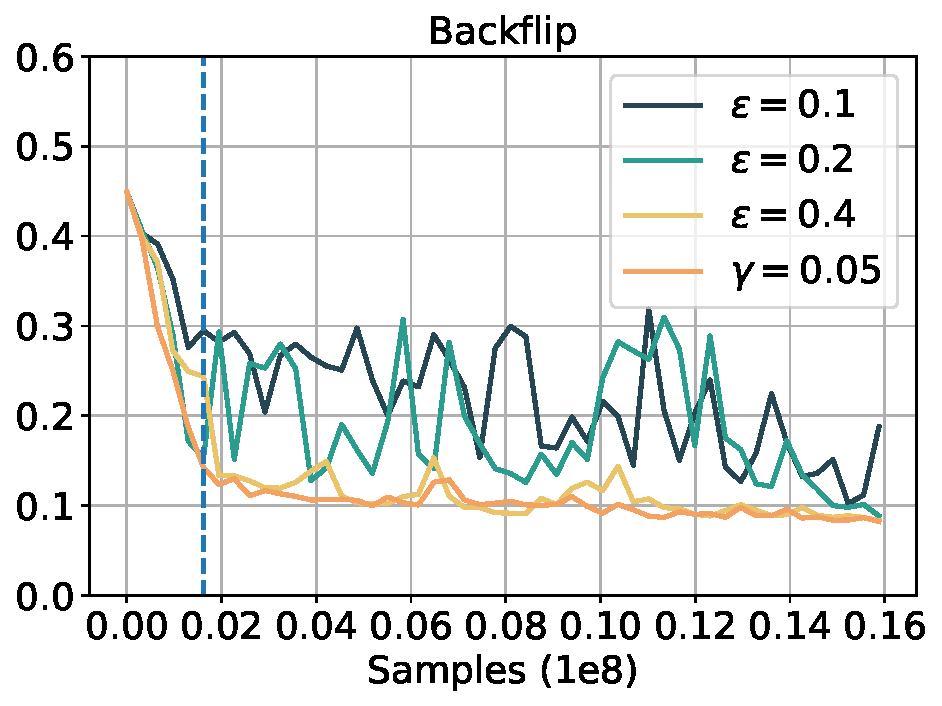
\includegraphics[width=0.3\textwidth]{figures/err_backflip.pdf}
    \\
    (a)
    &
    (c)
    &
    (e) 
    \\
    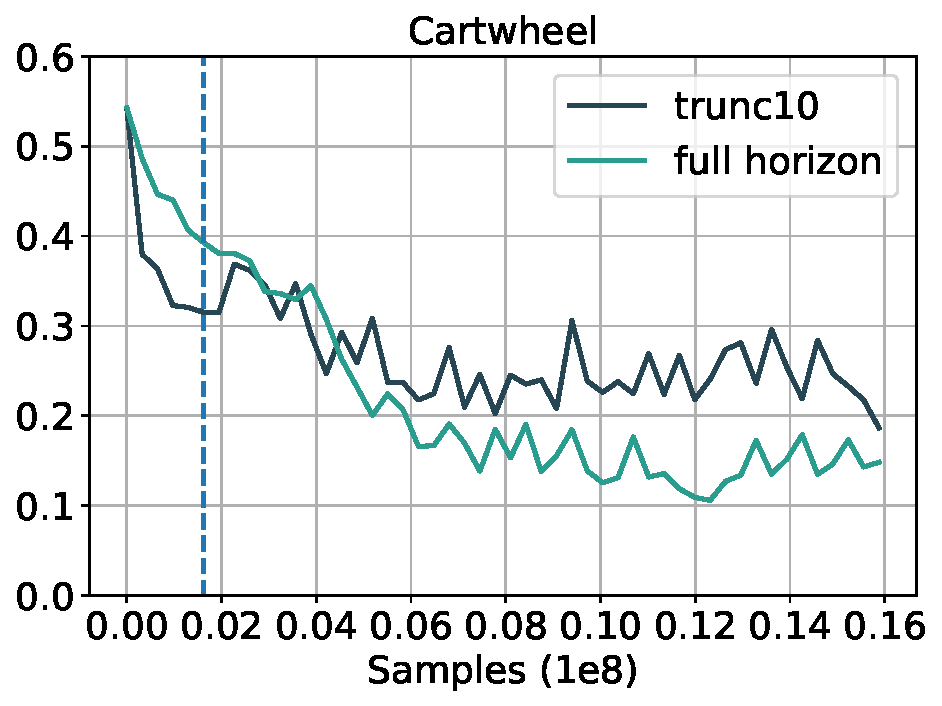
\includegraphics[width=0.3\textwidth]{figures/trunc_cartwheel.pdf}&
    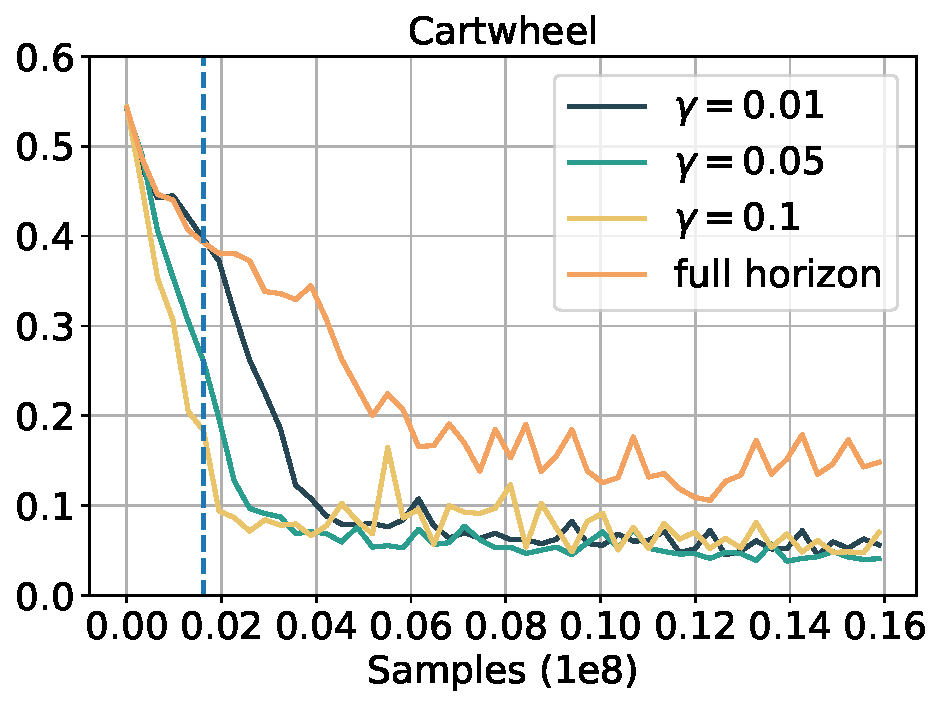
\includegraphics[width=0.3\textwidth]{figures/rand_cartwheel.pdf}&
    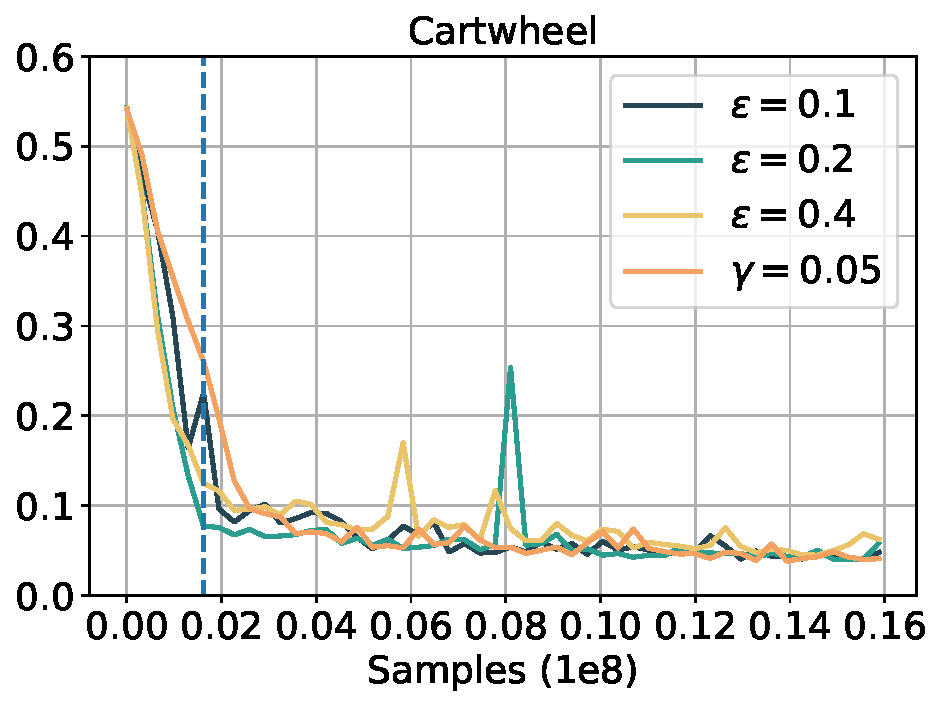
\includegraphics[width=0.3\textwidth]{figures/err_cartwheel.pdf}
    \\
    (b)
    &
    (d)
    &
    (f) 
    \end{tabular}
    \captionof{figure}{(a)-(b) Comparison between Full Horizon Gradient and truncation length of 10.
    (c)-(d)  Comparison between Demonstration Replay (Random) and Full Horizon Gradient.
    (e)-(f) Comparison between Demonstration Replay (Random) and Demonstration Replay (Threshold). The blue dotted line denotes 10 minutes in the corresponding wallclock time.}
    \vspace{-10pt}
    \label{tab:ablation}
\end{table}


To understand how demonstration replay affects the policy learning of DiffMimic, we compare three different variants of DiffMimic, namely, Demonstration Replay (Random) and Demonstration Replay (Threshold), and Full Horizon Gradient on \textit{Backflip} and \textit{Cartwheel}. Demonstration Replay (Random) randomly replaces a state in the rollout of the policy with the demonstration state at the same timestamp similar to the teacher forcing~\citep{williams1989learning}. Demonstration Replay (Threshold) inserts the demonstration state based on the pose error. If the pose error between the demonstration state and the simulated state exceeds a threshold $\epsilon$, the simulated state will be replaced by the demonstration state.
The Full Horizon Gradient variant backpropagates the gradient through the full horizon without any additional operation. We show the quantitative result in Fig.~\ref{tab:ablation}, and the qualitative result in Fig.~\ref{fig:vis_ablation}. 

\textbf{Demonstration replay helps stabilize policy learning and leads to better performance.} Compared with the Full Horizon Gradient without demonstration replay, the learning curve with demonstration replay is much smoother and finally converges to a lower pose error as shown in Fig.~\ref{tab:ablation} (c)-(d). We show in Fig.~\ref{fig:vis_ablation} (b), this vanilla version of DiffMimic can easily get stuck into a local minimum. Instead of learning to backflip, the policy learns to bend down and use arms to support itself instead of jumping up. The other two variants, by contrast, both learn to jump and backflip in mid-air successfully. 

\begin{wrapfigure}[19]{r}{0.38\columnwidth}
     \centering
     \vspace{-10pt}
     \centering
     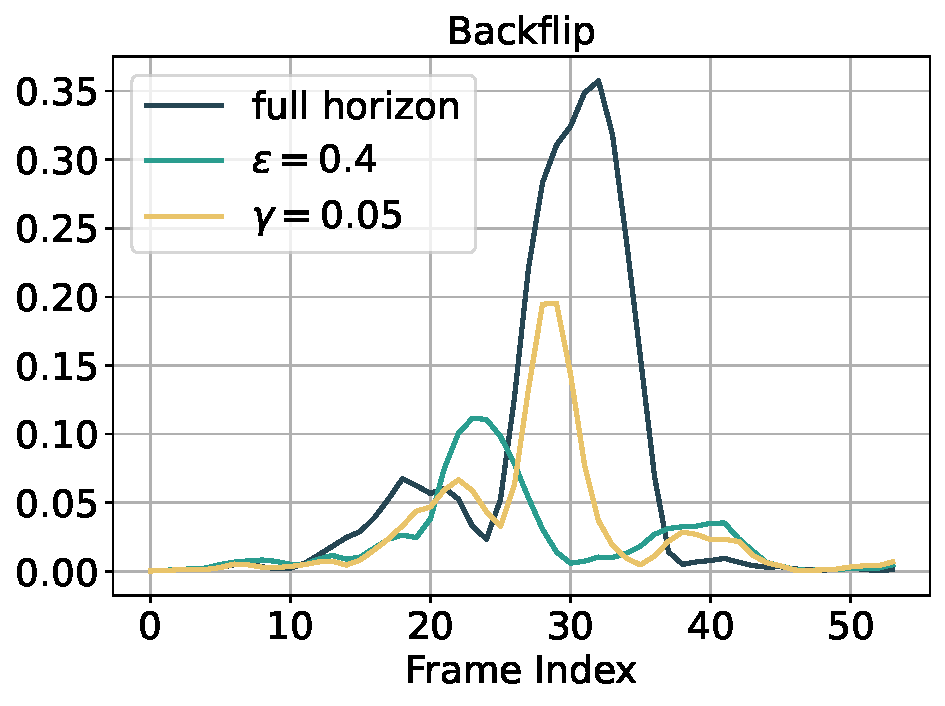
\includegraphics[width=0.38\textwidth]{figures/frame_backflip.pdf}
    \caption{L2 error per frame in the rollout of the final policy. Although Demonstration Replay (Random) reduces the overall pose error compared to full-horizon optimization, the per-frame loss remains large in certain time steps due to the lack of a constraint. Demonstration Replay (Threshold) alleviates the issue.}
    \label{fig:frame_loss}
\end{wrapfigure}
\textbf{Policy-aware demonstration replay leads to a more faithful recovery of demonstration.} 
We compare Demonstration Replay (Threshold) with Demonstration Replay (Random) in Fig.~\ref{tab:ablation} (e)-(f). Quantitatively, both variants yield similar results if the hyperparameter is properly tuned. However, the behavior of policies trained with these two strategies can be significantly different. In Fig.~\ref{fig:vis_ablation} (c) and (d), though both policies learn to backflip successfully, the policy trained with Demonstration Replay (Random) fails to recover the motion frame by frame. 
We show in Fig.~\ref{fig:frame_loss} the per-frame pose error. Even though the average error over the whole trajectory for both variants is similar, Demonstration Replay (Threshold) gives a lower maximum per-frame error, which indicates a faithful recovery of the demonstration. This implies that simply minimizing the pose error may not suffice to learn a policy that tracks the demonstration closely. Finer-grained guidance based on the current performance of the policy is required. 


















\section{Conclusion \& Future works}

In summary,  we present DiffMimic utilizes differentiable physics simulators (DPS) for motion mimicking and outperforms several commonly used RL-based methods in various tasks with high accuracy, stability, and efficiency. We believe DiffMimic can serve as a starting point for motion mimicking with DPS and that our simulation environments provide exciting opportunities for future research.

While there are many exciting directions to explore, there are also various challenges. One such challenge is to enable motion mimicking within minutes given any arbitrary demonstration. With differentiable physics, this would greatly accelerate downstream tasks. In our work, we demonstrate that DiffMimic can learn challenging motions in just 10 minutes. However, the tasks we evaluated were relatively short and did not involve any interactions with other objects. As the dynamic system becomes more complex with multiple objects, we leave these challenges for future work.



\clearpage
\section*{Ethics Statements}
We have carefully reviewed and adhered to the ICLR Code of Ethics. DiffMimic conducts experiments exclusively on humanoid characters, and no experiments involve human subjects. Additionally, all experiments are performed using open-sourced materials and are properly cited.

\section*{Reproducibility Statements}
Our code is easily accessible and openly available for review at \hyperlink{https://github.com/diffmimic/diffmimic}{https://github.com/diffmimic/diffmimic}. Additionally, the reported results can be easily reproduced using the provided code.

\section*{Acknowledgment}
This research is supported by the National Research Foundation, Singapore under its AI Singapore Programme (AISG Award No: AISG2-PhD-2022-01-036T,  AISG2-PhD-2021-08-015T and AISG2-PhD-2021-08-018), NTU NAP, MOE AcRF Tier 2 (T2EP20221-0012), and under the RIE2020 Industry Alignment Fund - Industry Collaboration Projects
(IAF-ICP) Funding Initiative, as well as cash and in-kind contribution from the industry partner(s).

{
    \small
    \bibliographystyle{ieeenat_fullname}
    \bibliography{main}
}


% WARNING: do not forget to delete the supplementary pages from your submission 
\clearpage
\setcounter{page}{1}
\maketitlesupplementary


\section{Relationship with MonoNeRF \cite{mononerf}}
\label{sec:relationship with mononerf}
We discuss the relationship between our strongest baseline MonoNeRF\cite{mononerf} and our proposed method MonoSelfRecon as follows: 1) We share the same idea of SFM-based 3DR with monocular RGB sequence as input, and we both jointly train SFM and a generalizable NeRF, where the NeRF is used to boost SFM performance.  2) Although using SFM as the core of framework design, we regress to different 3D representations, where MonoNeRF regress to view-based 2D depth map while we regress to 3D voxel-based SDF values. 3) While MonoNeRF also jointly estimates camera poses, their 2D view-based depth representation restricts the ability to incrementally complete a whole scene in 3D mesh representation. Fusing TSDF from direct depth estimation is time-consuming, and will cause layered or sparse mesh due to depth inconsistency between each frame. By comparison, our direct voxel-SDF regression enables us to incrementally add the previous mesh to complete the whole scene consistently in mesh representation.  

The mesh representation is a stricter 3D representation over 2D depth map. Theoretically, the depth map can be perfectly rendered from 3D mesh but cannot in reverse, which is further validated by our experiments. Table \ref{table:scannet} and \ref{table:7scenes} show that although all using ground truth for supervised training, the one that directly regresses SDF (NeuralRecon) has a clear advantage on 2D depth metrics over other supervised methods that regresses depth. The reason that although both our method and MonoNeRF are based on SFM while ours outperforms theirs can be also partly attributed to this different 3D representation. Our visual results also reflect this point in Table \ref{fig:visual results}, where although there is no much difference of 2D depth, the difference of 3D mesh is clear. In other words, the depth representation is more visually straightforward than 3D mesh. Consequently, our 3D mesh regressing is a stricter 3D geometric representation than MonoNeRF's 2D depth.


\section{Evaluation Metrics}
We follow the same evaluation metrics as \cite{atlas, neucon}. Details of the metrics are summarized in Table \ref{table:metrics}.
\begin{table}[htb]
\tiny
\setlength\tabcolsep{0.1pt}
\begin{tabular*}{\columnwidth}{@{\extracolsep{\fill}} llll}
\hline
\multicolumn{2}{l}{2D} & \multicolumn{2}{l}{3D} \\ \hline
Abs Rel             & $\frac{1}{n}\sum\left|d-d^*\right|/d^*$      & Acc       & $\text{mean}_{p \in P}\left(\min_{p^* \in P^*}||p-p^*||\right)$\\
Abs Diff            & $\frac{1}{n}\sum\left|d-d^*\right|$          & Comp      & $\text{mean}_{p^* \in P^*}\left(\min_{p \in P}||p-p^*||\right)$\\
Sq Rel              & $\frac{1}{n}\sum\left|d-d^*\right|^2/d^*$    & Prec      & $\text{mean}_{p \in P}\left(\min_{p^* \in P^*}||p-p^*||<.05\right)$\\
RMSE                & $\sqrt{\frac{1}{n}\sum\left|d-d^*\right|^2}$ & Recal     & $\text{mean}_{p^* \in P^*}\left(\min_{p \in P}||p-p^*||<.05\right)$\\
$\tiny\mkern-5mu\sigma<1.25$   & $\frac{1}{n}\sum\left(\max\left(\frac{d}{d^*}, \frac{d^*}{d}\right)<1.25\right)$ & F-score  & $\frac{2 \times \text{Prec} \times \text{Recal}}{\text{Prec} + \text{Recal}}$\\
Comp                & \% valid predictions &                        &                 \\
RMSE log            & $\sqrt{\frac{1}{n}\sum\left|\log(d)-\log(d^*)\right|^2}$   &                        &                 \\
Sc Inv              & $\left(\frac{1}{n}\sum_{i}z_i^2-\frac{1}{n^2}(\sum_i z_i)^2\right)^{1/2}$ &                        &                 \\ \hline
\end{tabular*}
\caption{\textbf{Evaluation Metrics.}}
\label{table:metrics}
\end{table}


\section{Model Details}
\subsection{Attentional View Fusion}
We use a standard Vision Transformer (ViT) Encoder, where we keep the original high-level architecture of the ViT encoder to be: A norm layer, a multi-head attention layer, a norm layer, and a MLP (2 heads are used). Originally the ViT takes image patch/features as input, while we adopted the input to be the nearest 2D features from the projected 3D voxels, which is of size $[N_{view}, N_{points}, C]$, where $N_{view}$ is the number of views in a scene fragment, $N_{points}$ is the number of voxels in a fragment, $C$ is the feature channel. The input also takes the voxel mask as input to filter out the pixels which are invisible to the voxels, and the transformer only takes the visible pixel features. We stack two ViT encoders to update the features, where the output is still of size $[N_{view}, N_{points}, C]$. Then we use a multi-view weighted feature pooling to fuse the updated features at the view channel to 3D features of size $[N_{points}, C]$, where the weight is the number of visible views in a fragment for each voxel. Such design enables more flexibility to adjust the contribution of each view to the 3D voxels. 

\subsection{GRU}
We directly use the GRU module from \cite{neucon}, which is elaborately designed for sparse 3D convolution. The 3D voxel features are obtained by attentional view fusions and fed to the GRU module, where the current 3D fragment features are conditioned on the previous fragment. Using the current 3D global voxel features $G^l_{t}$ and the previous hidden state $H^l_{t-1}$ at layer $l$,  the current hidden state $H^l_{t}$ can be obtained, and the SDF value at each level is regressed from the hidden state $H^l_{t}$. More specifically,

\begin{equation}
\begin{aligned}
     &z_t = \sigma(SparseConv([H^{l}_{t-1}, G^l_t], W_z)) \\
     &r_t = \sigma(SparseConv([H^{l}_{t-1}, G^l_t], W_r)) \\
     &\Tilde{H^l_t} = tanh(SparseConv([r_t \odot H^l_{t-1}, G^l_t], W_h)) \\
     &H^l_t = (1-z_t)\odot H^l_{t-1} + z_{t} \odot \Tilde{H^l_t}
\end{aligned}
\end{equation}

\noindent where $z_t$ is the update gate, $r_t$ is the reset gate, $\sigma$ is the sigmoid function and $W_{*}$ is the weight for sparse convolution. 






We first train without GRU within each fragment to warmup the framework with our proposed self-supervised losses, where we call it \textbf{intra-fragment losses}. Because the GRU module is leveraged to enhance the consistency between fragments, the self-supervised learning strategy should be treated differently to intra-fragment losses. There is no need to change the training policy in purely supervised training because SDF ground truth is used, and there is no ground truth in our self-supervision except for the consistency clues between fragments. So we extend the \textbf{inter-fragment losses} to \textbf{intra-fragment losses}. While the model only takes input per fragment, backpropagating whole fragments brings memory challenges, so we only implement the inter-fragment losses on the frames around the boundary of fragments. Specifically, we use the last 4 and first 4 frames of the previous and current fragments to implement the inter-fragment loss.

\begin{figure}
    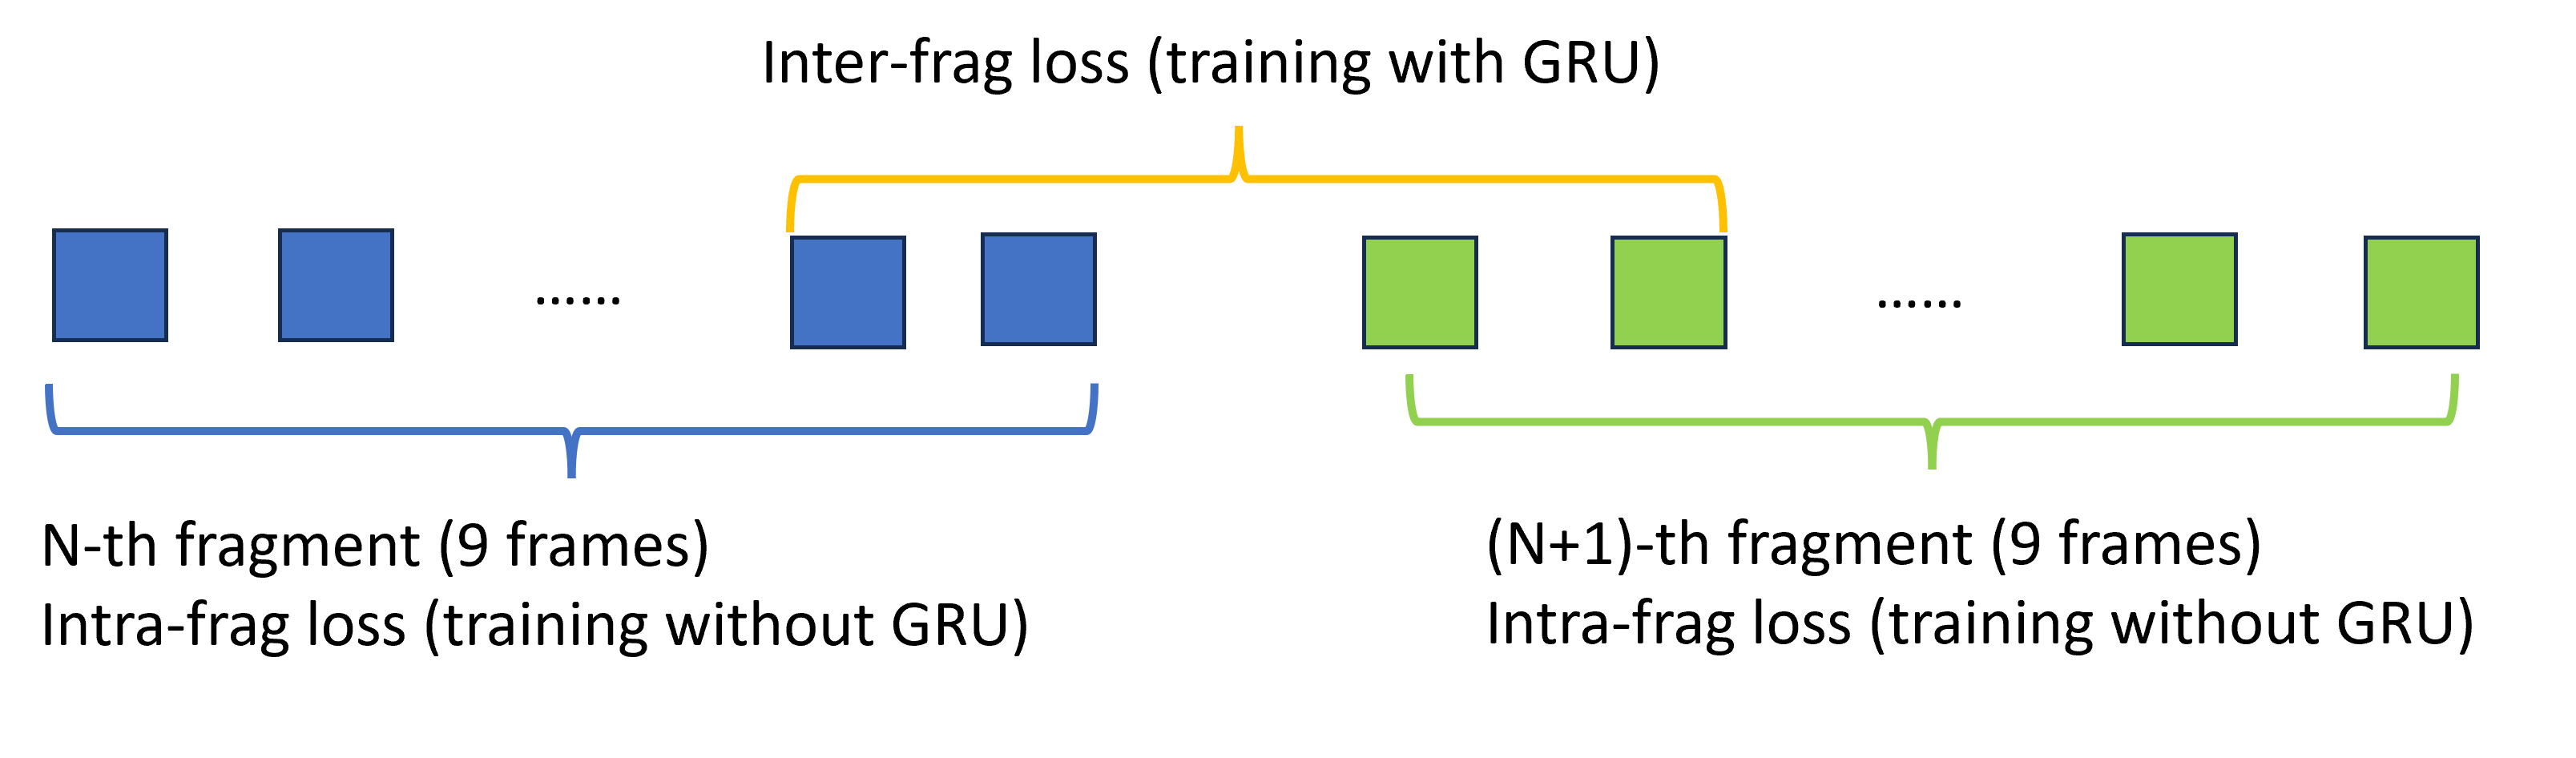
\includegraphics[width=\linewidth]{figures/GRUloss_explain.png}
    \caption{\textbf{Inter/Intra-fragment} losses illustration.}
    \label{fig:gruloss_explain}
\end{figure}


\subsection{NeRF}

\begin{figure}
    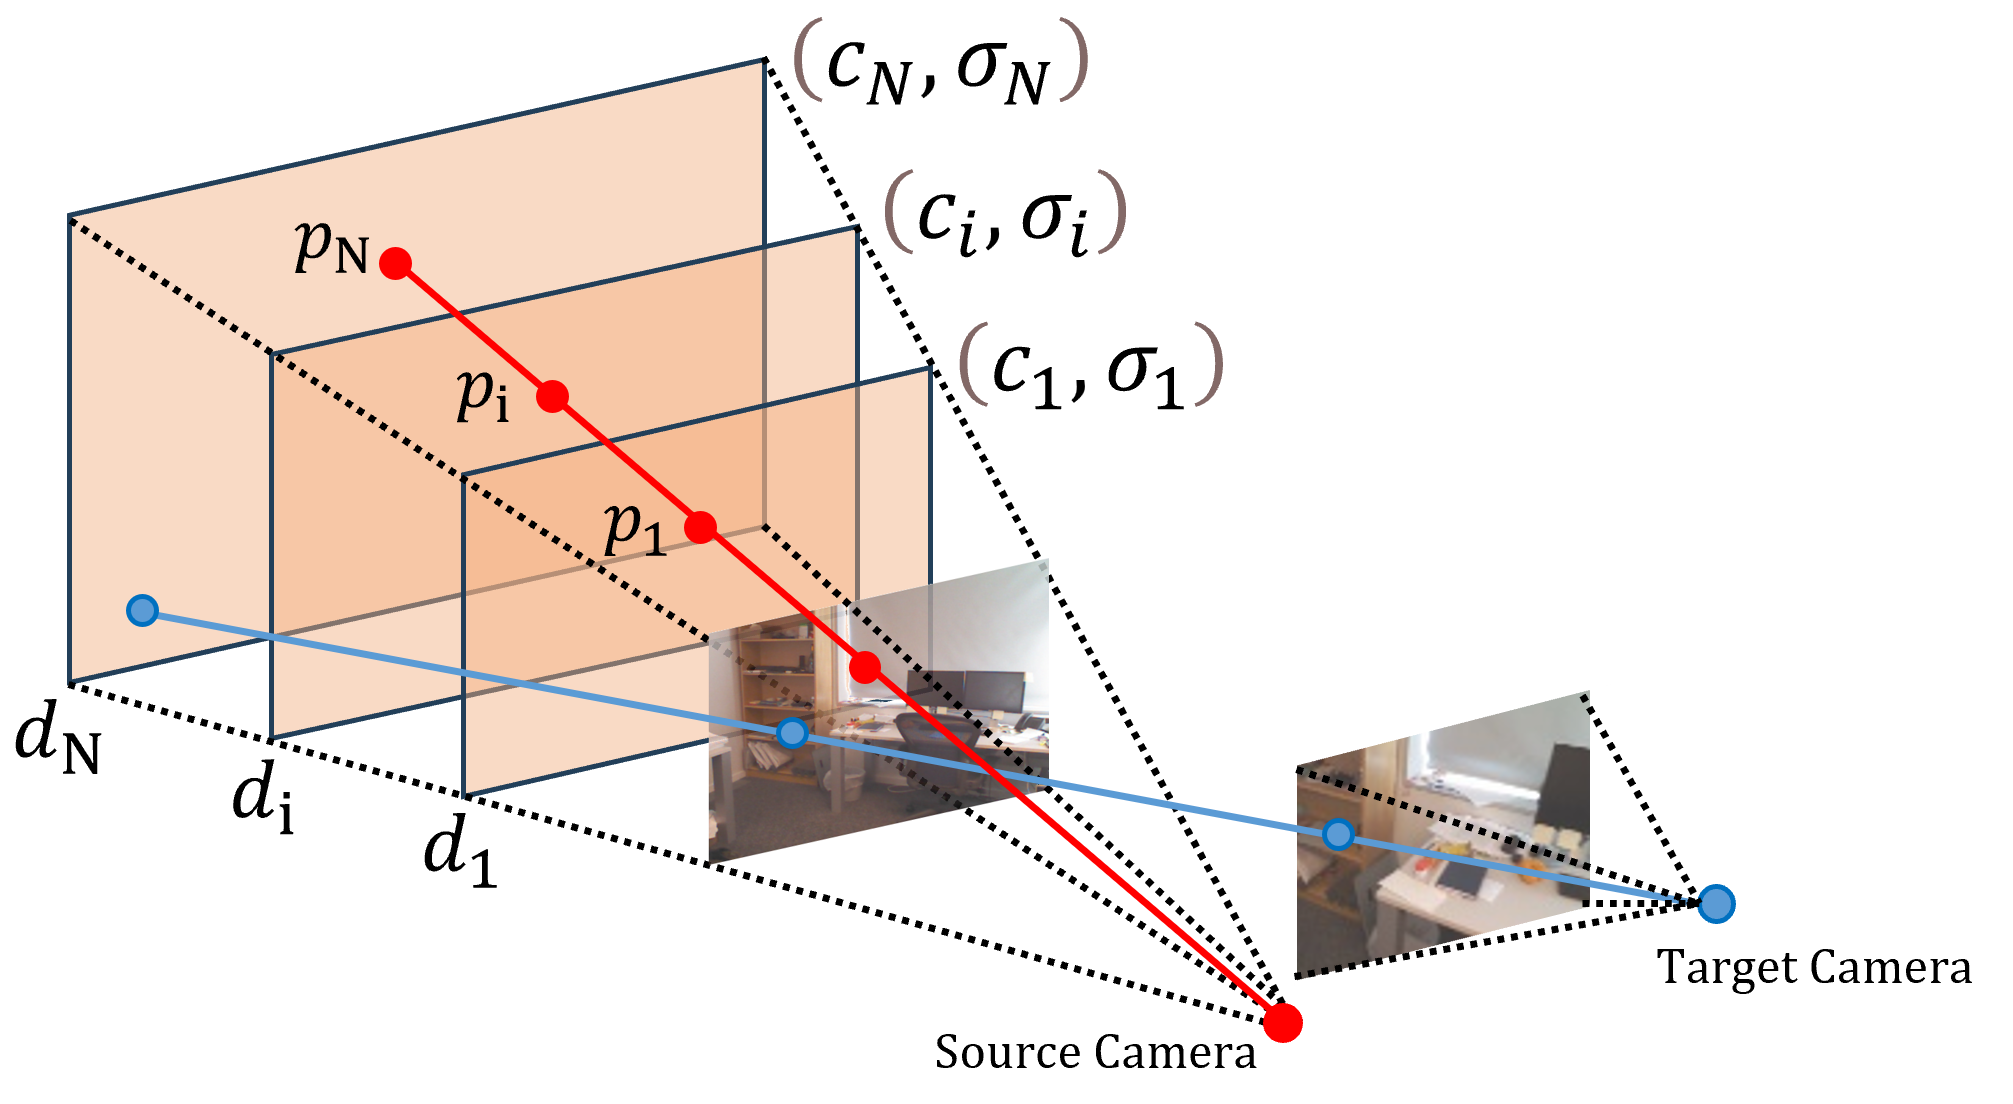
\includegraphics[width=\linewidth]{figures/MPI_explain.png}
    \caption{\textbf{Multi-Plane Image (MPI)} NeRF illustration.}
    \label{fig:mpi_explain}
\end{figure}


Since the SDF decoder is generalizable, the NeRF also must be generalizable to boost SDF decoder. For our work, we adopted MPI-NeRF\cite{mpi, mpi-nerf}, which has been directly used by MonoNeRF\cite{mononerf} and proved to be generalizable. As Figure \ref{fig:mpi_explain} shows, in Multi-Plane-Image (MPI) system, an image is represented by a set of parallel planes (orange planes) denoted as RGB-$\sigma$, specifically $(c_{i}, \sigma_{i})_{i=1}^N$,  where the $i_{th}$ plane has $d_{i}$ disparity (reverse of depth) to the camera. The shading points (red points) are selected as the intersection of the parallel planes and the rays shooting from pixels in the image, where $c_{i}$ and $\sigma_{i}$ are the RGB color and density of each shading points at $i_{th}$ plane. In a standard MPI system, the source view RGB image $\hat{I_{s}}$ and depth map $\hat{D_{}}$ can be composed using the ``over'' operation \cite{over_composite} as

\iffalse
\begin{equation}
    \Biggl\{ \begin{array}{cc}
     \hat{I}_{s} = \sum_{i=1}^{D}(c_{i}\sigma_{i}\prod_{j=i+1}^{D}(1-\sigma_{j})) \\
     \\
     \hat{D}_{s} = \sum_{i=1}^{D}(d_{i}^{-1}\sigma_{i}\prod_{j=i+1}^{D}(1-\sigma_{j}))
     \end{array}
\end{equation}
\fi


{
\begin{equation}
\begin{aligned}
    \hat{I}_s &= \sum_{i=1}^{D} (c_i \sigma_i \prod_{j=i+1}^{D} (1 - \sigma_j)) \\
    \hat{D}_s &= \sum_{i=1}^{D} (d_i^{-1} \sigma_i \prod_{j=i+1}^{D} (1 - \sigma_j))
\end{aligned}
\label{eq:combined}
\end{equation}
}

To use MPI system in NeRF style, the composition operation above can be replaced by volumetric rendering \cite{nerf} for both RGB and depth as 
\iffalse
\begin{equation}
    \Biggl\{ \begin{array}{cc}
    \hat{I_s} = \sum_{i=1}^{N}T_{i}(1-exp(-\sigma_{i}\delta_{i}))c_{i} \\
    \\
    \hat{Z_s} = \sum_{i=1}^{N}T_{i}(1-exp(-\sigma_{i}\delta_{i}))z_{i}
    \end{array}
\end{equation}
\fi

{
\begin{equation}
\begin{aligned}
    \hat{I}_s &= \sum_{i=1}^{N}T_{i}(1-exp(-\sigma_{i}\delta_{i}))c_{i} \\
    \hat{Z}_s &= \sum_{i=1}^{N}T_{i}(1-exp(-\sigma_{i}\delta_{i}))z_{i}
\end{aligned}
\label{eq:combined}
\end{equation}
}

\noindent where $z_i$ is the rendered depth (reverse of disparity) $z_i = 1/d_i$, and $\delta_i = ||p_{i+1} - p_i||_2$ is the distance between the two neighbor shading points on a ray. Then we can extend volumetric rendering to target views. First, the corresponding pixels $[u_t, v_t]$ in the target view can be found by 

\begin{equation}
    \begin{bmatrix}
        u_{s} \\
        v_{s} \\
        1
    \end{bmatrix}
    \sim K_{s}(R-tn^{T}d_{i})(K_{t})^{-1}
    \begin{bmatrix}
        u_{t} \\
        v_{t} \\
        1
    \end{bmatrix}
\end{equation}

Here, $[u_s, v_s]$ is the corresponding pixel locations in the source view, $K_s$ and $K_t$ are camera intrinsics of source and target views, $R$ and $t$ are rotation and translation from the target to source view, and $n$ is the norm vector of the $i_{th}$ plane. As the planes are parallel, the RGB $c'_i$ and density $\sigma'_i$ of shading points (blue points) on target rays (blue ray) are equal to those from source rays at the same disparity, as shown in Eq. \ref{mpinerf_samergbsigma},

\iffalse
\begin{equation}
    \Biggl\{ \begin{array}{cc}
    c_{i}'(u_{t}, v_{t}) = c_{i}(u_{s}, v_{s}) \\
    \sigma_{i}'(u_{t}, v_{t}) = \sigma_{i}(u_{s}, v_{s})
    \end{array}
    \label{mpinerf_samergbsigma}
\end{equation}
\fi

{
\begin{equation}
\begin{aligned}
    c_{i}'(u_{t}, v_{t}) = c_{i}(u_{s}, v_{s}) \\
    \sigma_{i}'(u_{t}, v_{t}) = \sigma_{i}(u_{s}, v_{s})
\end{aligned}
\label{mpinerf_samergbsigma}
\end{equation}
}

\iffalse
\begin{equation}
    \Biggl\{ \begin{array}{cc}
     \hat{I}_{t} = \sum_{i=1}^{D}(c_{i}'\sigma'_{i}\prod_{j=i+1}^{D}(1-\sigma_{j}')) \\
     \\
     \hat{D}_{t} = \sum_{i=1}^{D}(d_{i}\sigma'_{i}\prod_{j=i+1}^{D}(1-\sigma_{j}'))
     \end{array}
\end{equation}
\fi

Once we have RGB and density for target views, we can perform volumetric rendering on target views as: 
\iffalse
\begin{equation}
    \Biggl\{ \begin{array}{cc}
    \hat{I_t} = \sum_{i=1}^{N}T_{i}(1-exp(-\sigma'_{i}\delta_{i}))c'_{i} \\
    \\
    \hat{Z_t} = \sum_{i=1}^{N}T_{i}(1-exp(-\sigma'_{i}\delta_{i}))z'_{i}
    \end{array}
\end{equation}
\fi

{
\begin{equation}
\begin{aligned}
    \hat{I_t} = \sum_{i=1}^{N}T_{i}(1-exp(-\sigma'_{i}\delta_{i}))c'_{i} \\
    \hat{Z_t} = \sum_{i=1}^{N}T_{i}(1-exp(-\sigma'_{i}\delta_{i}))z'_{i}
\end{aligned}
\label{eq:combined}
\end{equation}
}

We use standard NeRF RGB loss, where $\hat{I}_s$ and $\hat{I}_t$ are self-supervised with their corresponding input images with a L1 loss. Since we directly use the reverse of disparity for depth, the depth value is scale-ambiguous. As mentioned in the paper, since there is no depth ground truth for pure self-supervision, we use SDF-depth as pseudo-depth to first recover the real scale of $\hat{Z}_s$ and $\hat{Z}_t$, then we impose a consistency loss between $\hat{Z}$ and SDF-depth to boost SDF decoder.

    

\section{Visual Results}
We show more visual results of 2D rendered depth and 3D mesh in Figure \ref{fig:scannet_supp}. \textbf{We also attach a PowerPoint file with visual results, where reviewers can rotate and zoom the 3D mesh to see the details},

\section{Limitation}
Although our work combines the advantages of ``self-supervised'' ``generalizable'' and ``3D explicit mesh'' altogether, there are still limitations. So far our MonoSelfRecon can be only used for indoor environments, because we pre-define the 3D scene fragment with a fixed voxel number. Unlike indoor 2D images where depth vary within few meters, the depth can vary significantly just within a single 2D image in outdoor. It is applicable to keep the voxel number while increasing the voxel size, but it will lead to very poor resolution within voxels, which misses most of the details. Moreover, since we regress SDF corresponding to the discrete $N\times N\times N$ voxels of scene fragment, we cannot directly estimate SDF of a continuous 3D space, unless by interpolation. By contrast, SDF-NeRF based methods estimate SDF values in continuous 3D space but it is not generalizable to another scene. Our future works will explore to make SDF-NeRF generalizable, so that the 3DR can be ``self-supervised", ``generalizable", ``explicit'', ``indoor/outdoor'', and ``continous in 3D space''. 

\newpage
\begin{figure*}
\begin{minipage}{\textwidth}
  \centerline{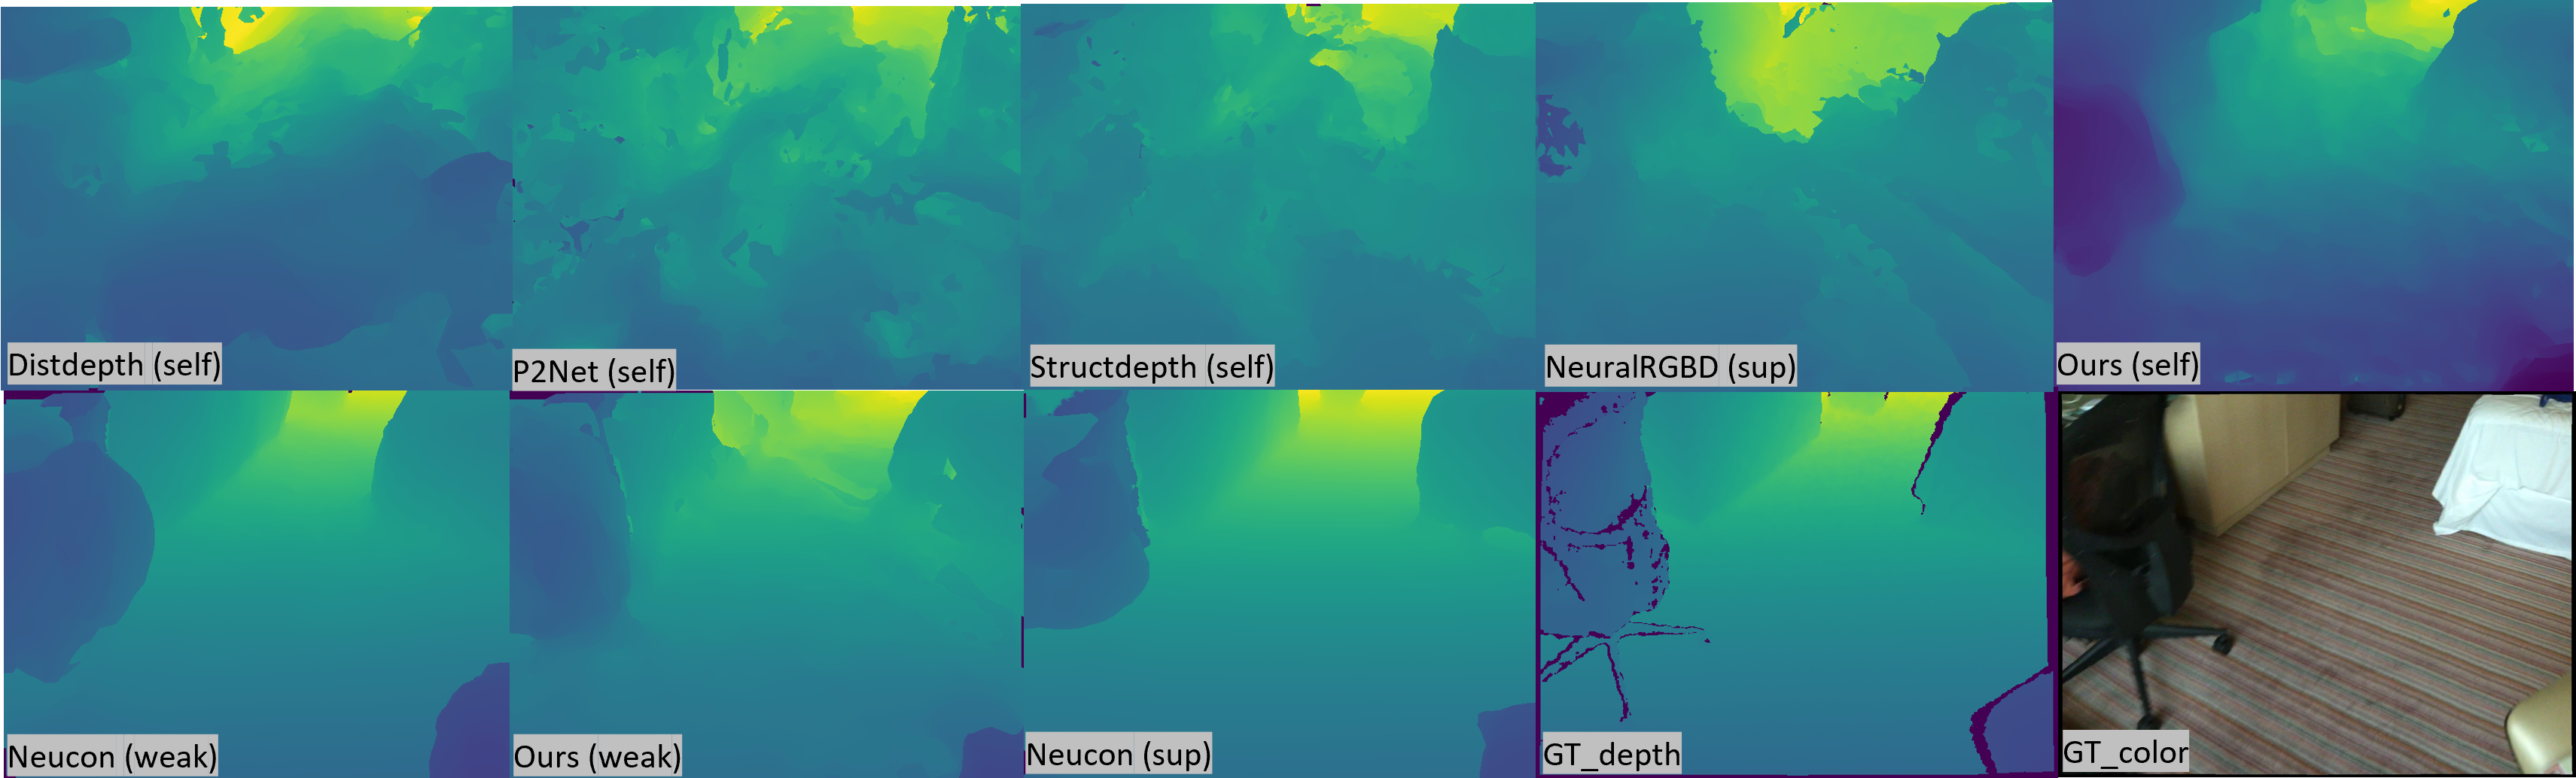
\includegraphics[width=1.0\textwidth]{figures/scannet_depth/738_1300.png}}
\end{minipage}
\vfill
\begin{minipage}{\linewidth}
  \centerline{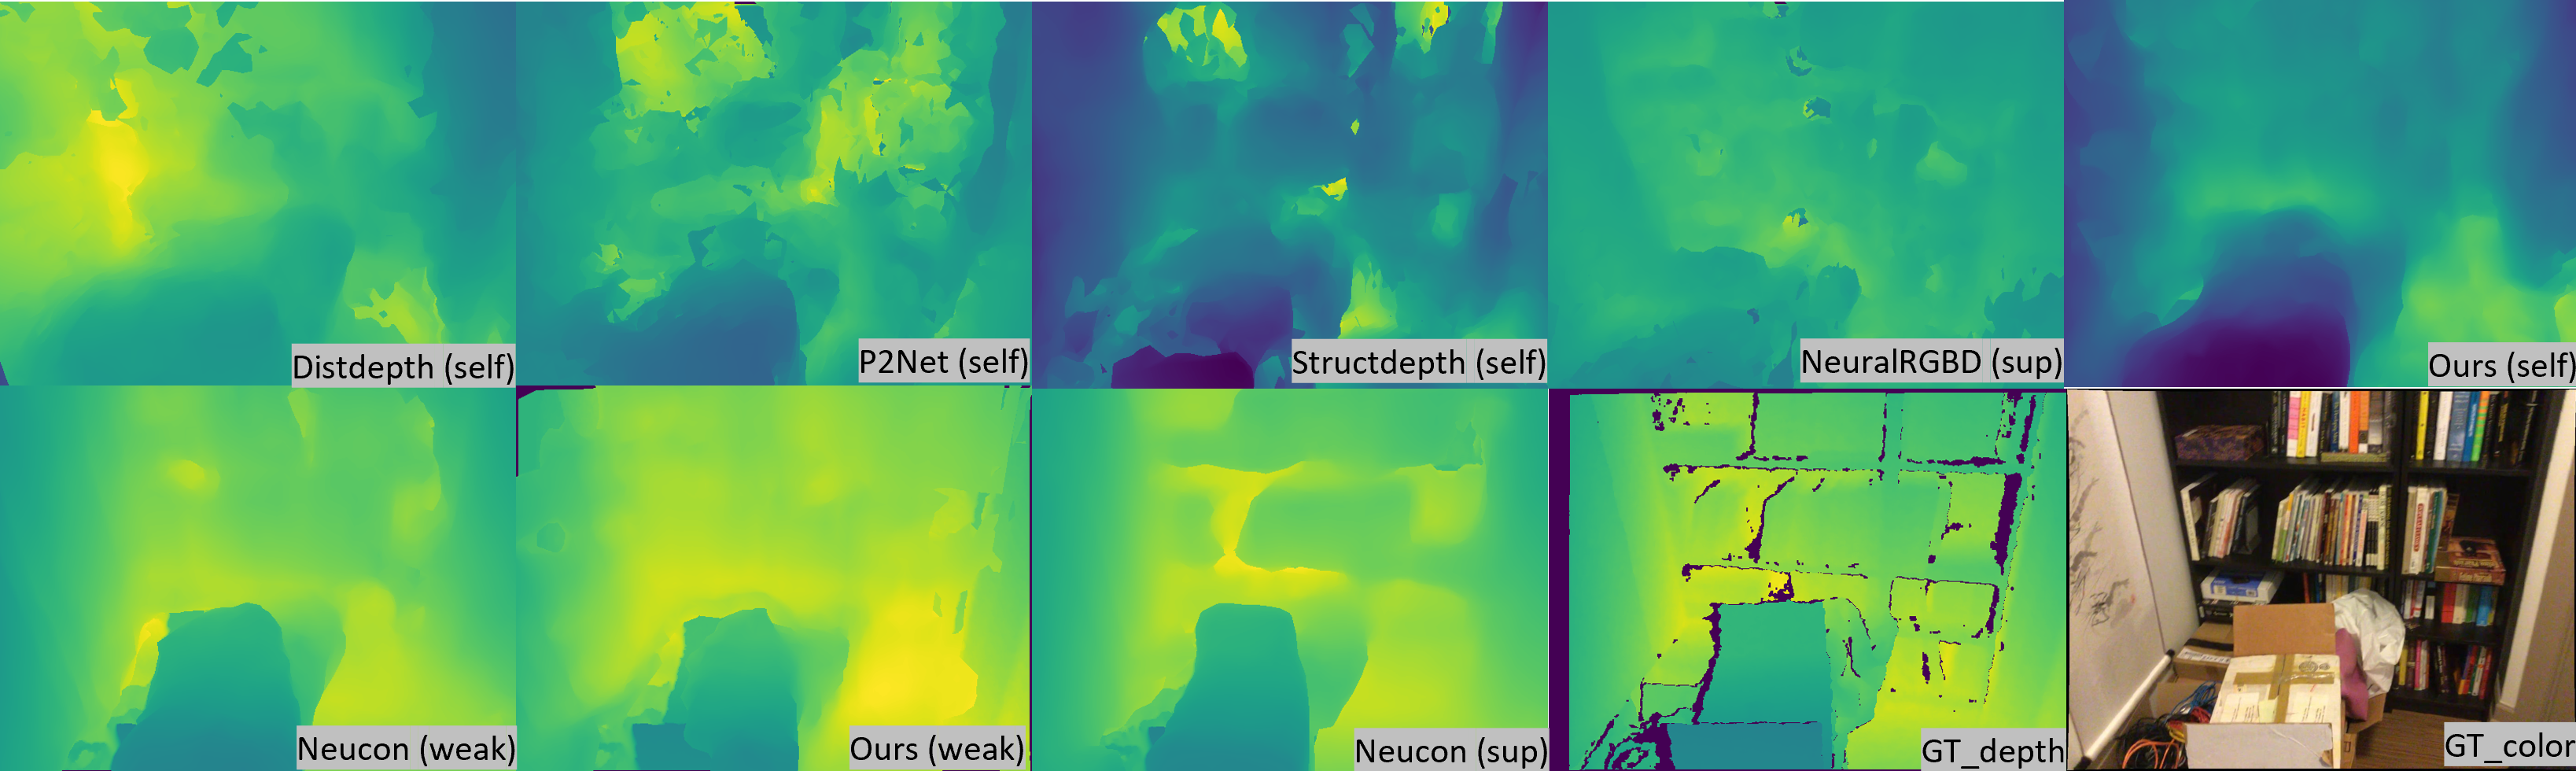
\includegraphics[width=1.0\textwidth]{figures/scannet_depth/710_1210.png}}
\end{minipage}
\vfill
\begin{minipage}{\linewidth}
  \centerline{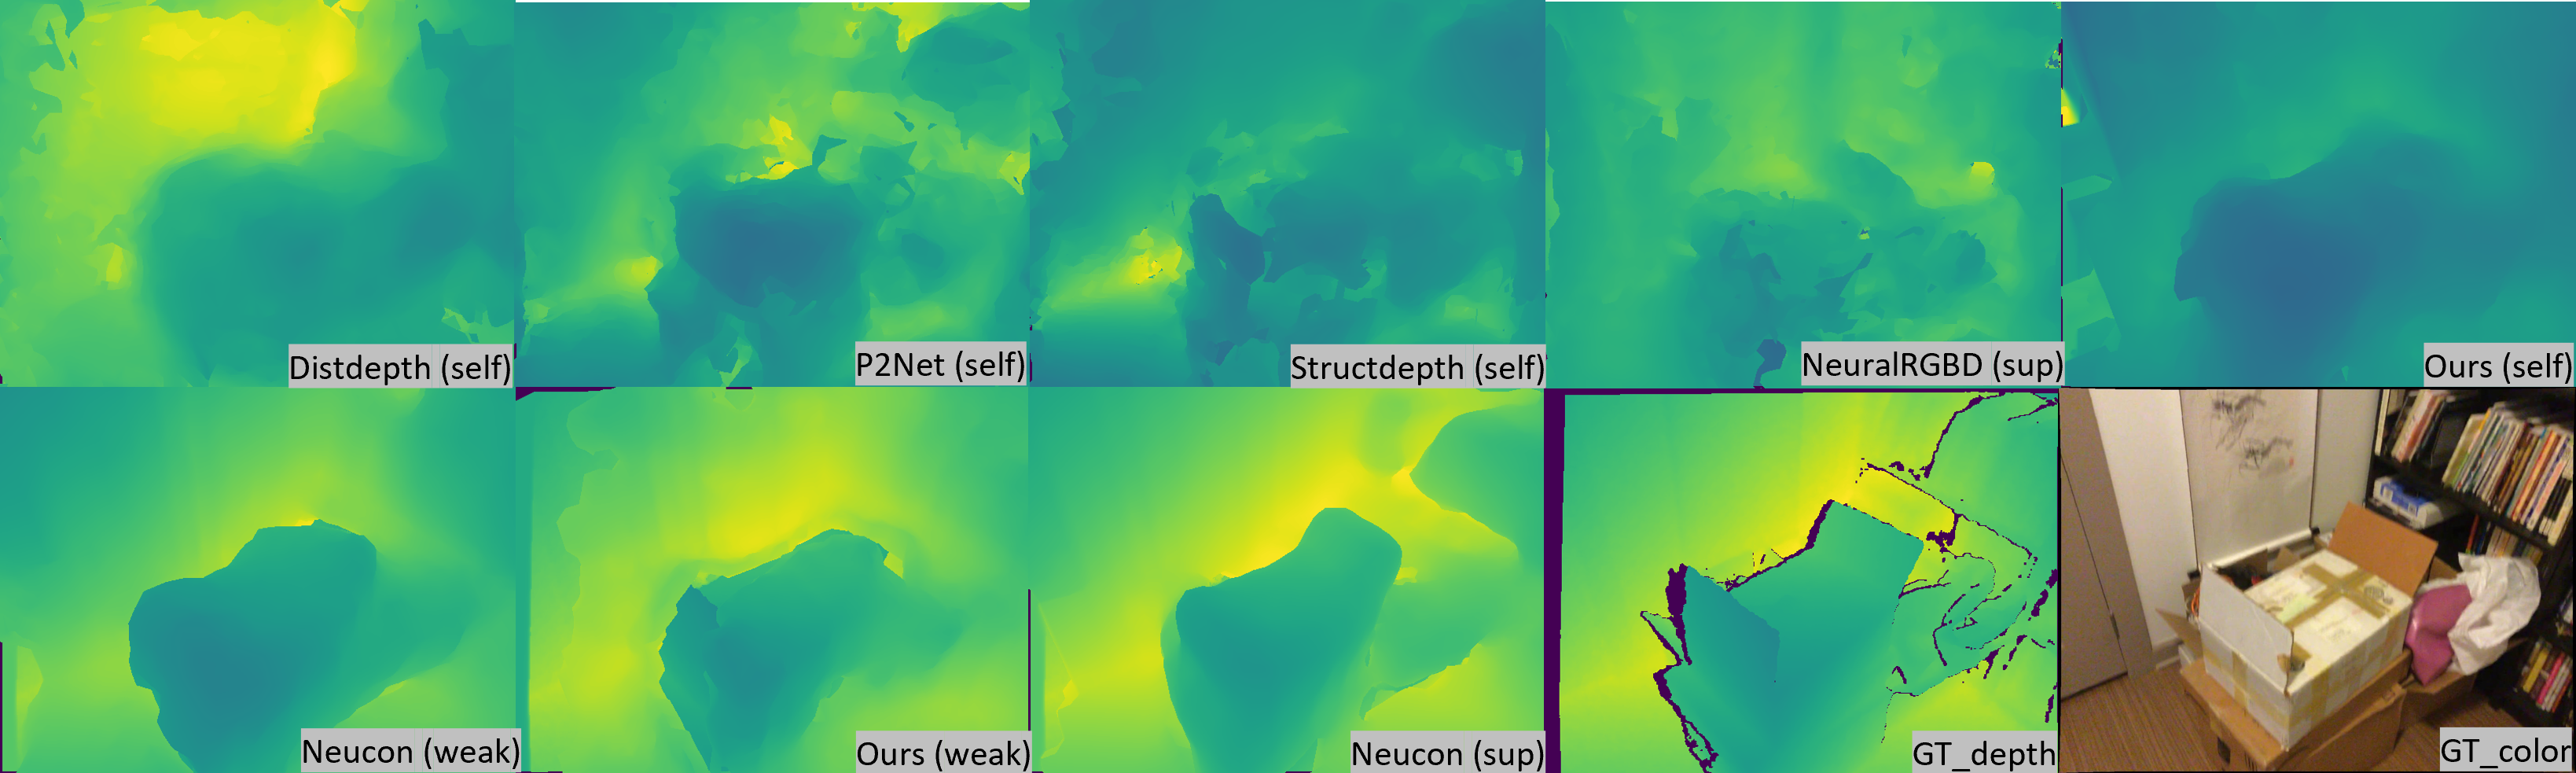
\includegraphics[width=1.0\textwidth]{figures/scannet_depth/710_1280.png}}
\end{minipage}
%\vspace{-3mm}
\begin{minipage}{\linewidth}
  \centerline{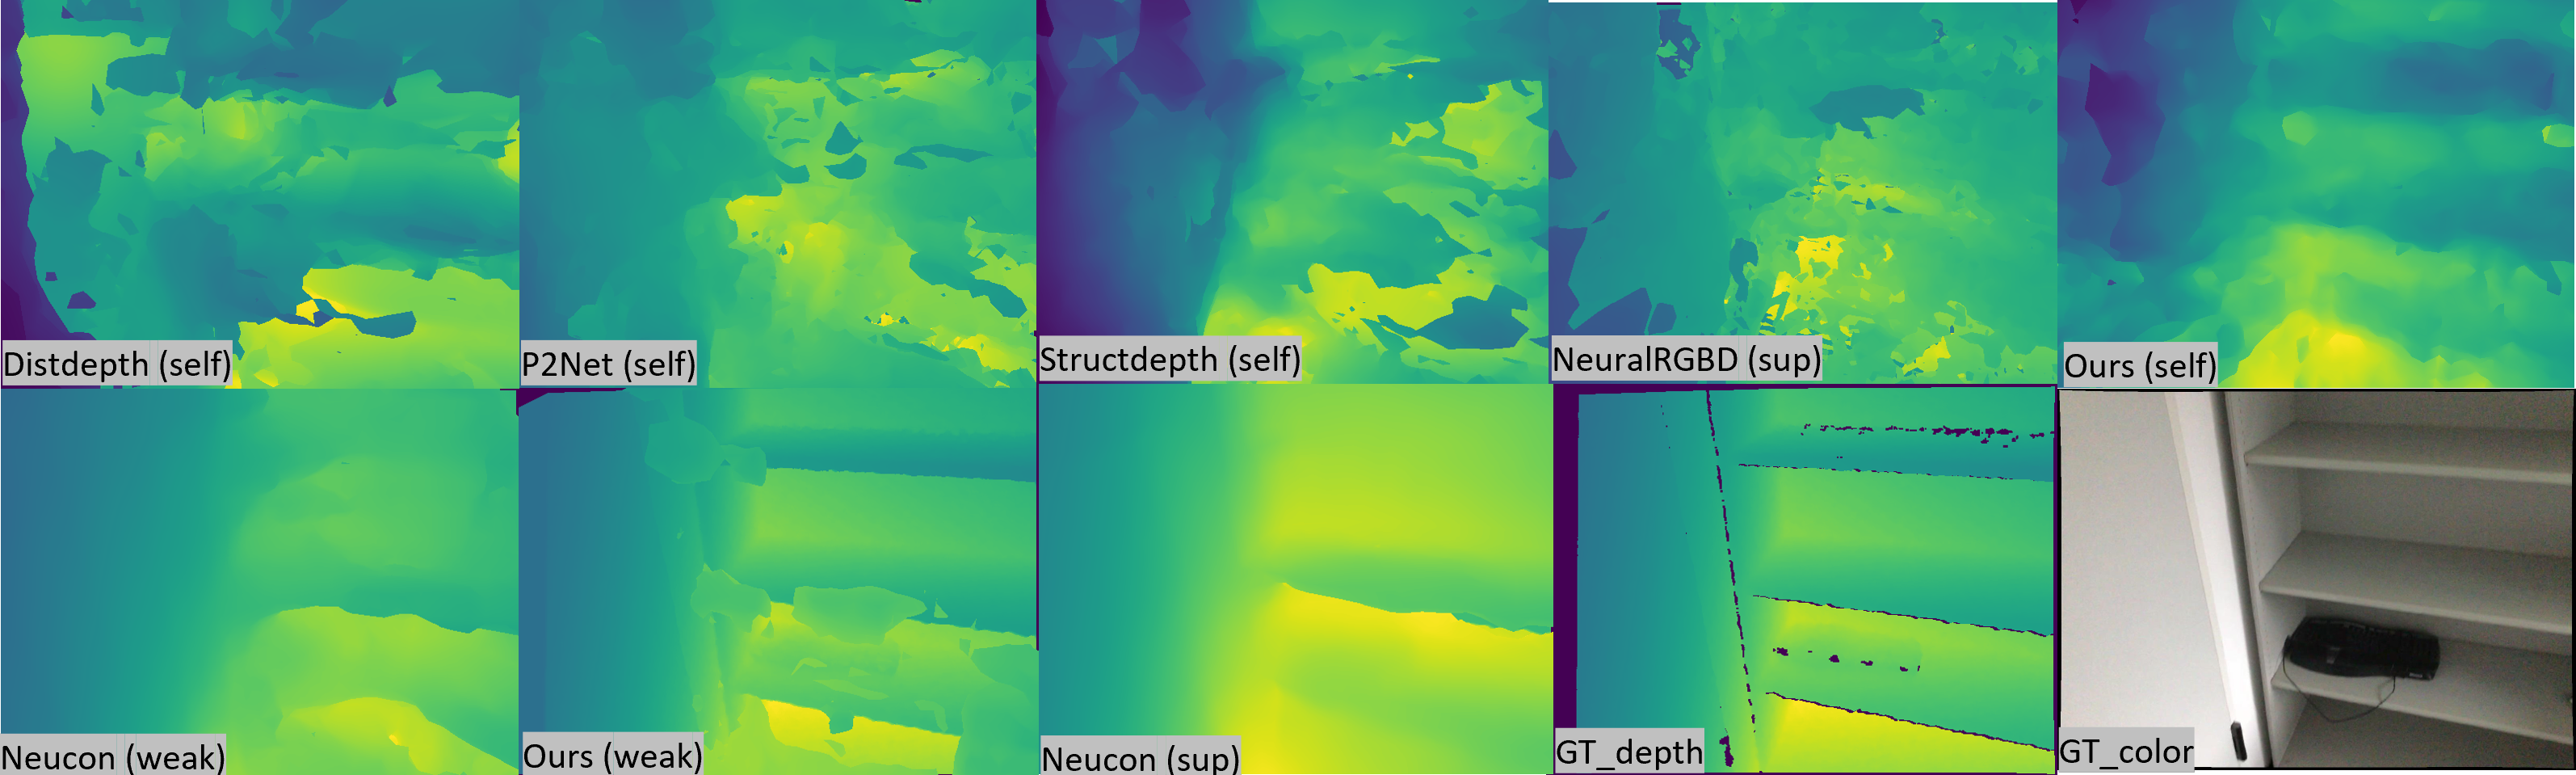
\includegraphics[width=1.0\textwidth]{figures/scannet_depth/711_880.png}}
\end{minipage}
%\vspace{-3mm}
\end{figure*}

\newpage
\begin{figure*}
\begin{minipage}{\textwidth}
  \centerline{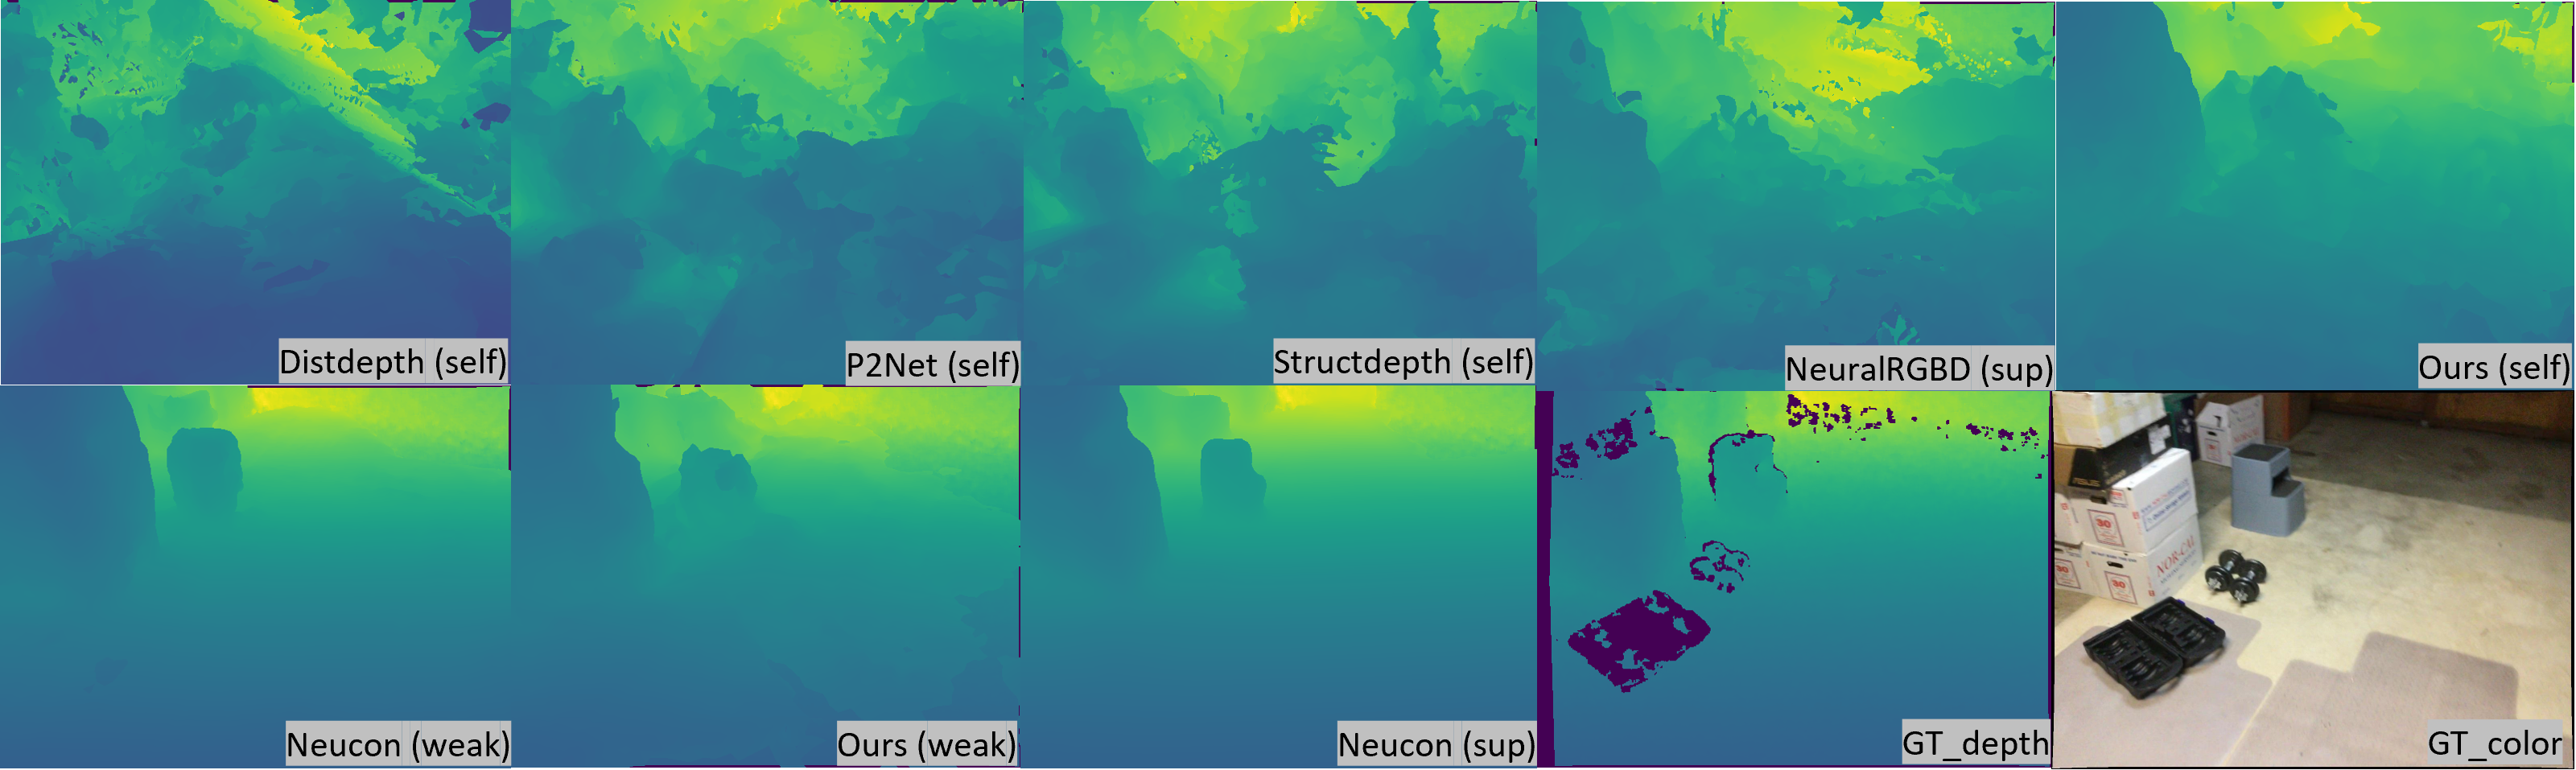
\includegraphics[width=1.0\textwidth]{figures/scannet_depth/787_1720.png}}
\end{minipage}
\vfill
\begin{minipage}{\linewidth}
  \centerline{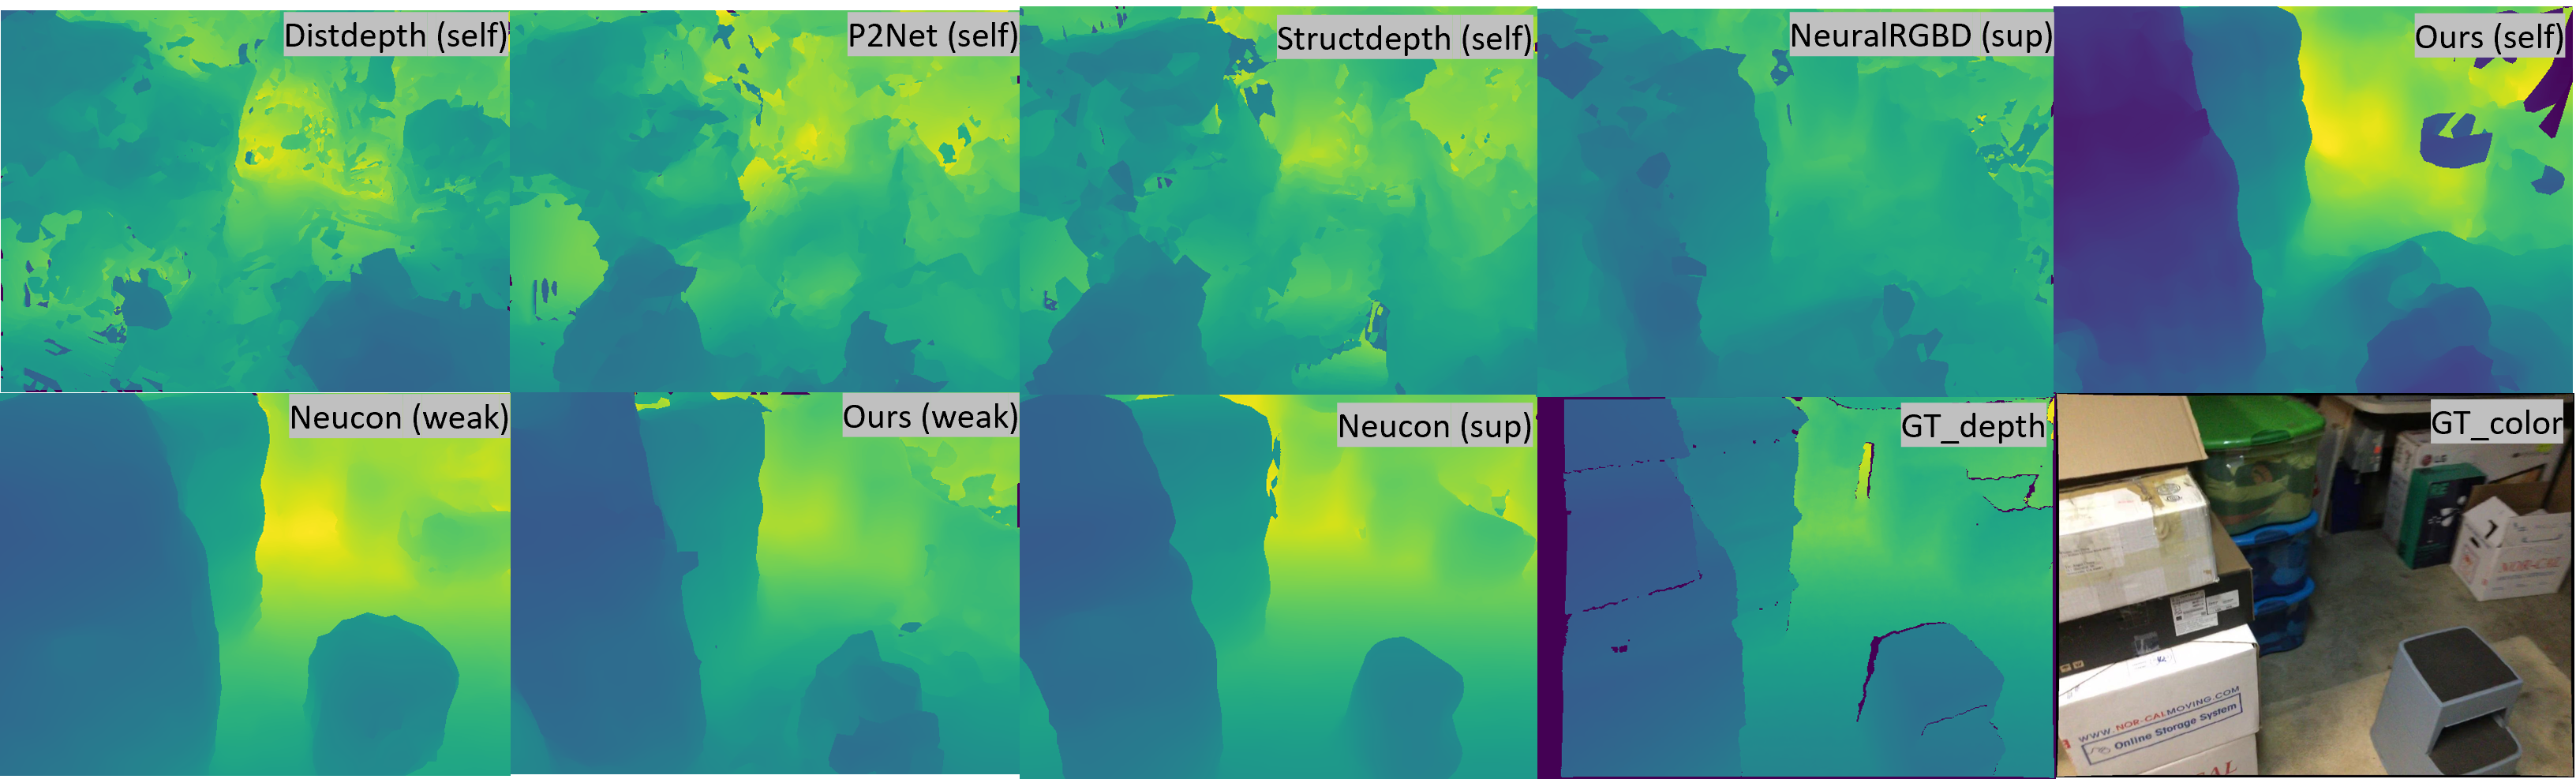
\includegraphics[width=1.0\textwidth]{figures/scannet_depth/787_1930.png}}
\end{minipage}
\vfill
\begin{minipage}{\linewidth}
  \centerline{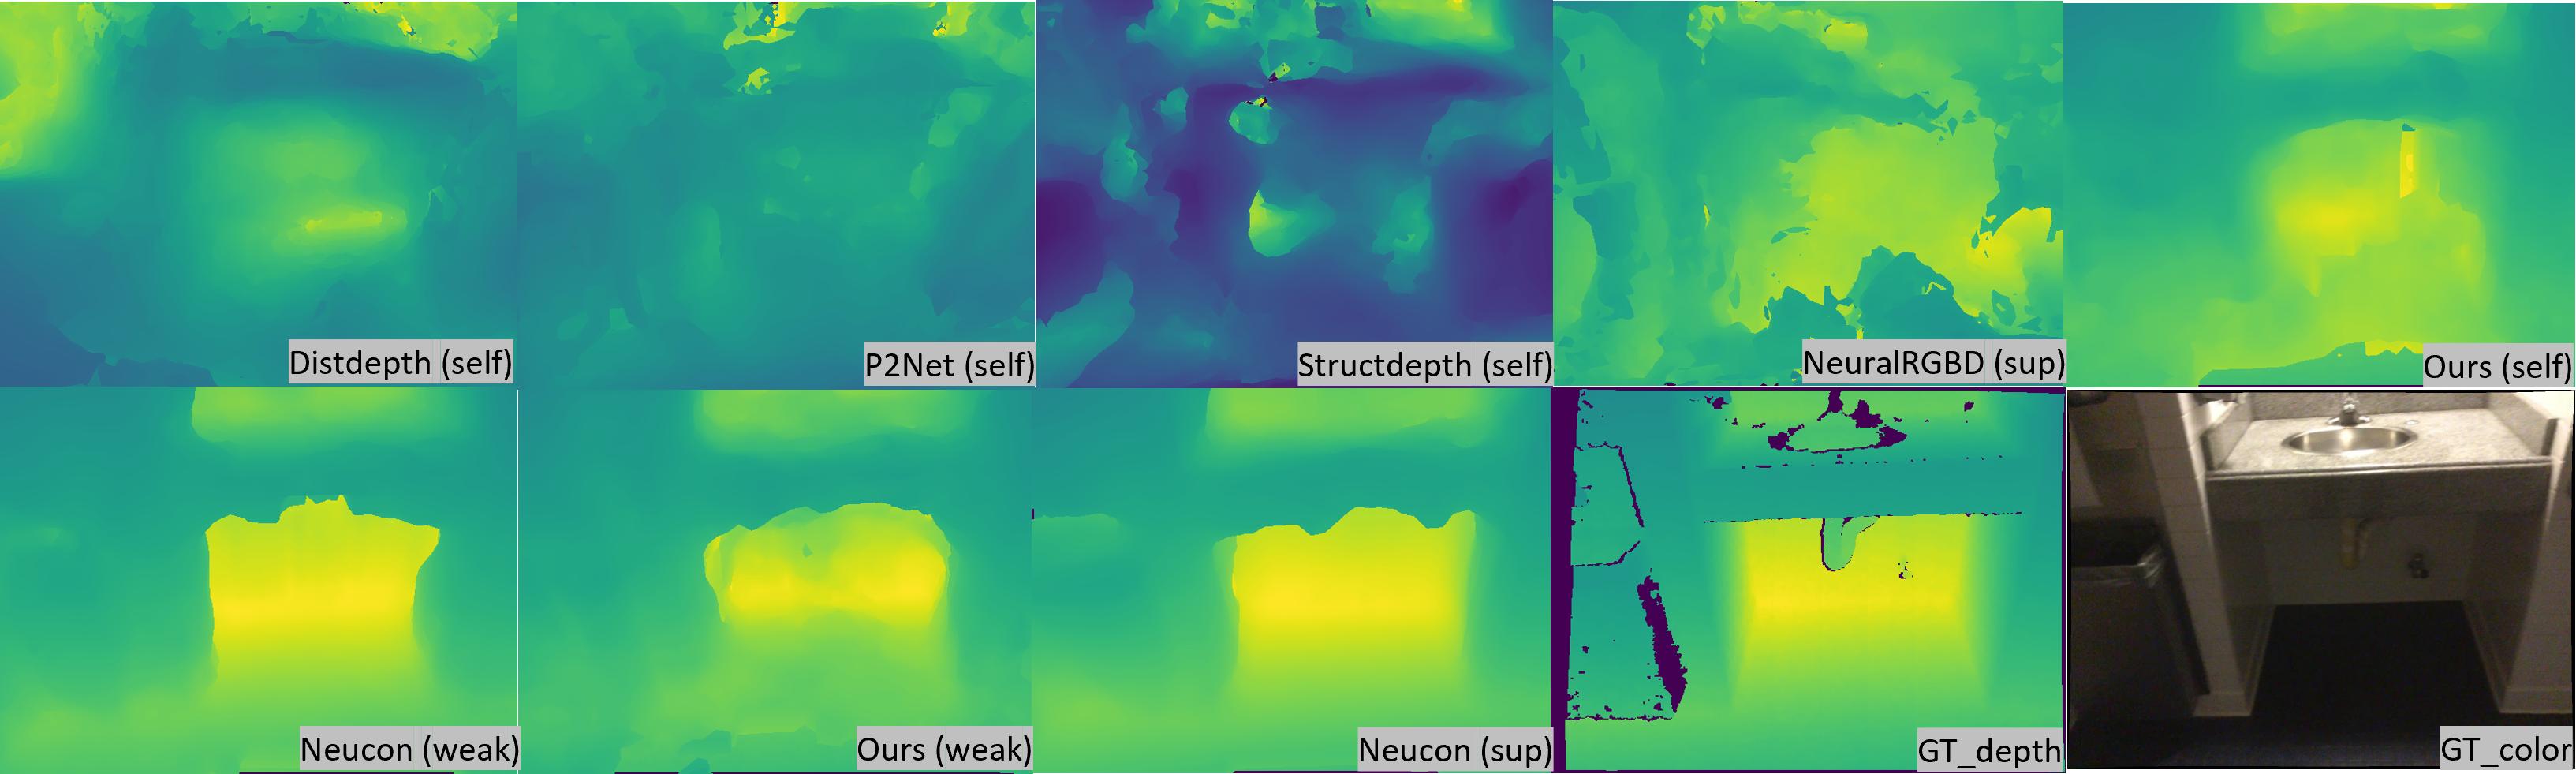
\includegraphics[width=1.0\textwidth]{figures/scannet_depth/779_1125.png}}
\end{minipage}
%\vspace{-3mm}
\begin{minipage}{\linewidth}
  \centerline{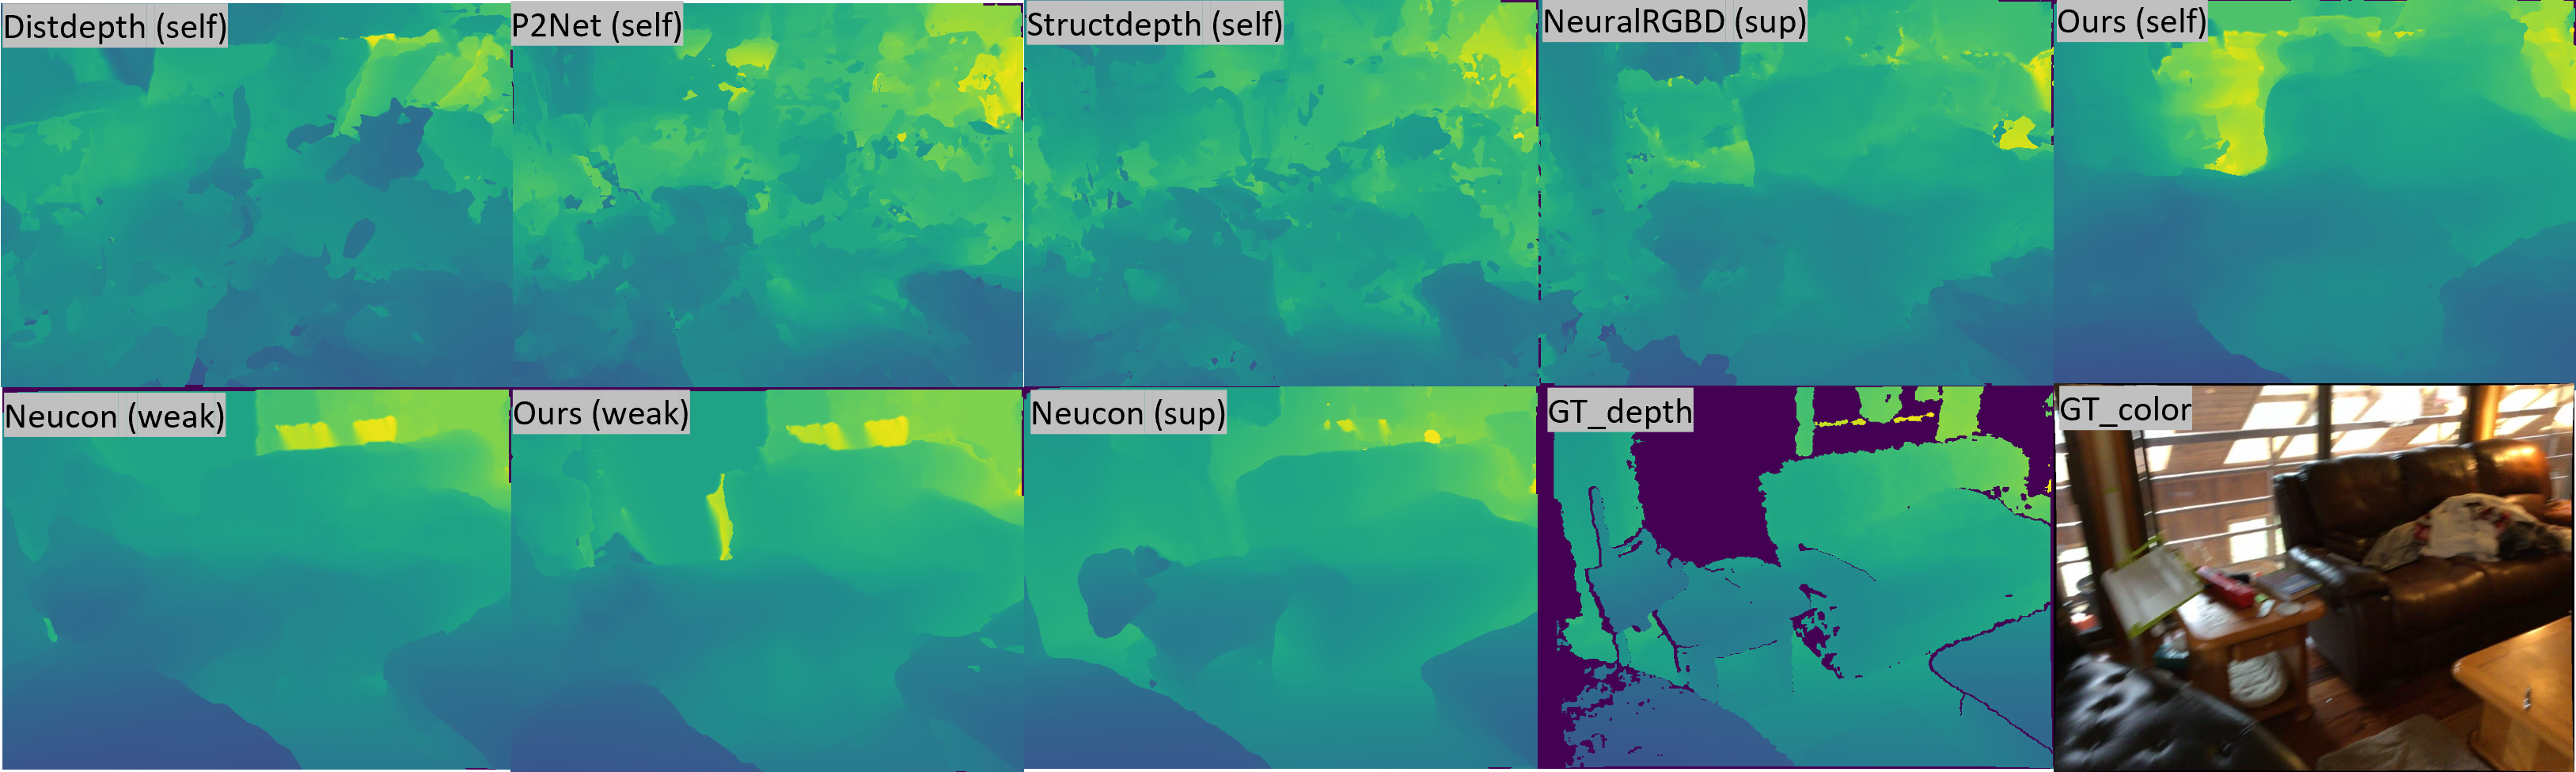
\includegraphics[width=1.0\textwidth]{figures/scannet_depth/747_97.png}}
\end{minipage}
%\vspace{-3mm}
\vspace{-3mm}
\end{figure*}

\newpage
\begin{figure*}
\begin{minipage}{\textwidth}
  \centerline{\includegraphics[width=1.0\textwidth]{figures/scannet_mesh/787.png}}
\end{minipage}
\vfill
\begin{minipage}{\linewidth}
  \centerline{\includegraphics[width=1.0\textwidth]{figures/scannet_mesh/747.png}}
\end{minipage}

\iffalse
\vfill
\begin{minipage}{\linewidth}
  \centerline{\includegraphics[width=1.0\textwidth]{figures/scannet_mesh/710.png}}
\end{minipage}
\fi
\label{fig:scannet_supp}
    \caption{Visual Results}
\end{figure*}


\end{document}
